\documentclass[11,5pt]{report}

%====================== PACKAGES ======================

\usepackage[french]{babel}
\usepackage{fancyhdr}
\usepackage[utf8]{inputenc}
%pour gérer les positionnement d'images
\usepackage{float}
\usepackage{lastpage}
\usepackage{graphicx}
\usepackage[colorinlistoftodos]{todonotes}
\usepackage{url}
%pour les informations sur un document compilé en PDF et les liens externes / internes
\usepackage{hyperref}
\usepackage[final]{pdfpages}
%espacement entre les lignes
\usepackage{setspace}
%modifier la mise en page de l'abstract
\usepackage{abstract}
%police et mise en page (marges) du document
\usepackage[T1]{fontenc}
\usepackage[top=2cm, bottom=2.5cm, left=2.5cm, right=2.5cm]{geometry}
%Pour les galerie d'images
\usepackage{subfig}
\pagestyle{fancy}
\fancyfoot[C]{\textbf{Page \thepage/\pageref{LastPage}}}
\usepackage{enumitem}

\renewcommand{\labelitemi}{$\bullet$}

%======================== DEBUT DU DOCUMENT ========================

\begin{document}
\begin{spacing}{2}
\newcommand{\HRule}{\rule{\linewidth}{0.5mm}}
\begin{titlepage}
\begin{center}

% Upper part of the page. The '~' is needed because only works if a paragraph has started.
\begin{figure}[h]
		\begin{minipage}[c]{.46\linewidth}
			\flushleft
			
\includegraphics[height=100 pt, width=120 pt]{images/ensias_logo.png}
		
		\end{minipage}
		\hfill%
		\begin{minipage}[c]{.46\linewidth}
			\flushright
			
\includegraphics[height=100 pt, width=120 pt]{images/um5.png}
		
		\end{minipage}
\end{figure}
\vspace{1cm}
\textsc{\Large École nationale supérieure d'informatique et d'analyse des systèmes}\\[0.3cm]

\textsc{\Large }\\[0.5cm]

% Title
\HRule \\[0.4cm]

{\huge \bfseries Rapport de Projet de Fin de 1\textsuperscript{ère} Année\\[0.2cm]}
{\huge \bfseries Création Automatique d'Histoires avec GPT-3 et Python\\[0.4cm]}

\HRule \\[1.5cm]

% Author and supervisor
\vspace{1cm}
\begin{minipage}{0.4\textwidth}
\begin{flushleft} \large
\emph{Réalisé par:}\\
\textsc{Ghita LOUKILI }\\
\textsc{Yahya NAHLI }\\
\end{flushleft}
\end{minipage}
\begin{minipage}{0.4\textwidth}
\begin{flushright} \large
\emph{Encadré par:} \\
\textsc{PR.Abdellatif \\EL FAKER}\\
\end{flushright}
\end{minipage}

\vfill

% Bottom of the page
{\large Année universitaire : 2022 - 2023}

\end{center}
\end{titlepage}

%page blanche
\newpage
\thispagestyle{empty}
~
\chapter*{Remerciements}
\addcontentsline{toc}{chapter}{Remerciements}
\large
\begin{onehalfspace}
Avant d'aborder plus en détail ce projet, nous souhaitons exprimer notre gratitude envers notre professeur, M. EL FAKER Abdellatif, qui nous a guidés avec patience et pédagogie tout au long de notre travail.

Nous tenons également à adresser nos remerciements spéciaux à nos autres professeurs pour leurs remarques, leurs directives et leur intérêt manifesté envers les étudiants. Nous les remercions sincèrement pour leur soutien et leur orientation précieux.
\end{onehalfspace}
\thispagestyle{empty}
\newpage

\chapter*{Résumé}
\addcontentsline{toc}{chapter}{Résumé}
\large
\begin{onehalfspace}
Ce projet académique porte sur les applications de l’intelligence artificielle, notamment la création automatique d’histoires en utilisant GPT-3 et Python. Le but est de permettre à un narrateur virtuel de raconter une histoire générée par un modèle linguistique, en se basant sur des paramètres fournis par l’utilisateur. Notre projet explore l’automatisation des étapes d’écriture, de division en scènes, de génération d’images et de la voix.

\textbf{Mots clés : } GPT-3, python, automatisation
\end{onehalfspace}
\thispagestyle{empty}
\newpage

\chapter*{Abstract}
\addcontentsline{toc}{chapter}{Abstract}
\large
\begin{onehalfspace}
This academic project explores the automation of story creation using AI. The goal is to develop a virtual narrator that can tell stories generated by a linguistic model, based on parameters provided by the user. The project explores the automation of the following stages :  writing, division into scenes, generation of images and of the voice.

\textbf{Keywords : } GPT-3, python, automation
\end{onehalfspace}
\thispagestyle{empty}
\newpage

\listoffigures
\thispagestyle{empty}
\tableofcontents
\thispagestyle{empty}
\newpage

%espacement entre les lignes d'un tableau
\renewcommand{\arraystretch}{1}

%====================== INCLUSION DES PARTIES ======================

\chapter*{Introduction générale}
\addcontentsline{toc}{chapter}{Introduction}

\begin{onehalfspace}
L'intelligence artificielle (IA) générative, avec des modèles avancés tels que GPT-3, a révolutionné le domaine de la narration et de la création d'histoires. Dans notre projet, nous avons exploité ces avancées pour développer un système automatisé de création et de narration d'histoires en utilisant GPT-3 et Python.

Notre objectif principal est de permettre aux utilisateurs de décrire brièvement une histoire en utilisant des indications sur les personnages, les lieux et les relations entre les personnages. En utilisant le modèle linguistique GPT-3, notre système génère ensuite une histoire complète, fidèle aux indications de l'utilisateur. De plus, des outils d'IA génèrent automatiquement les personnages, les paysages et le scénario, ajoutant une dimension visuelle à l'expérience de narration.

Dans ce rapport, nous décrirons les différentes étapes de notre projet. Le premier chapitre présentera le contexte du projet, les concepts clés de l'IA générative et du prompt engineering\cite{PromptGuide}. Le deuxième chapitre abordera les outils et ressources utilisés, tels que GPT-3, Lexica\cite{Lexica} et les outils de synthèse vocale.
Le troisième chapitre se concentrera sur les aspects techniques de la génération automatique d'images et de la création de la voix pour la narration. Enfin, nous partagerons les résultats obtenus, les limites rencontrées et les perspectives d'amélioration pour notre système de création et de narration d'histoires automatisé.

Ce projet nous permettra d'explorer les possibilités de l'IA générative, du traitement du langage naturel et de la génération d'images, tout en nous familiarisant avec des outils modernes.
\end{onehalfspace}


\chapter{Présentation du projet}
\section{Amenant}

\par 
Au cours de notre première année de formation en tant qu'élèves ingénieurs à l'ENSIAS, nous nous sommes lancés dans un projet ambitieux : la création automatique d'histoires en utilisant GPT-3 et Python. Notre objectif principal est de développer une application innovante qui tire parti des avancées de l'IA générative pour générer des histoires captivantes, accompagnées d'images et de voix immersives.

\section{Analyse de l'existant}

\par 
L'intelligence artificielle générative a révolutionné le domaine de la création d'histoires et d'images, ouvrant ainsi des perspectives passionnantes en termes de créativité et d'innovation. Grâce aux avancées des modèles d'apprentissage profond tels que GPT-3, la capacité à générer des récits cohérents et captivants a atteint des niveaux sans précédent. Ces modèles peuvent analyser de vastes quantités de données textuelles et apprendre les motifs, les styles et les structures propres à la narration, leur permettant ainsi de générer des histoires uniques et fascinantes. De plus, l'intelligence artificielle générative a étendu son champ d'action à celui des images, permettant la création de visuels réalistes et visuellement époustouflants. En utilisant des techniques telles que les réseaux antagonistes génératifs (GAN), les systèmes d'IA peuvent générer des images haute résolution, des peintures, voire même des modèles 3D d'une précision remarquable. Cette fusion de l'IA générative avec la narration et les arts visuels présente un potentiel immense dans divers secteurs tels que le divertissement, la publicité et les expériences de réalité virtuelle, vu qu'elle permet aux créateurs de produire un contenu riche et immersif en une fraction du temps traditionnellement requis.


\section{Problématique soulevée}
\par 
Après le développement de l'IA générative, un nouveau défi se pose : comment interagir efficacement avec ces IA ? Un domaine émergent, le prompt engineering\cite{PromptGuide}, est apparu pour répondre à ce besoin. Il consiste à formuler des instructions précises pour guider les modèles d'IA générative dans leurs réponses. Cependant, cela soulève des questions sur la formulation optimale des prompts, les implications éthiques liées aux biais potentiels et les limites de l'autonomie de l'IA.  

Nous sommes amenés à trouver la formulation  adéquate des prompts pour obtenir des récits cohérents et captivants, tout en guidant l'IA de manière précise.   De plus, il est essentiel de développer des techniques pour générer des images réalistes qui correspondent aux différentes scènes de l'histoire. 



\section{Solution proposée}

Notre projet consiste en 3 axes importants pour développer un système de génération automatique d'histoires en utilisant un modèle linguistique avancé. L'utilisateur aura la possibilité de donner de brèves indications sur les caractéristiques des personnages et les circonstances de l'histoire, afin de définir les thèmes principaux sur lesquels l'IA se basera. En exploitant ces indications, le modèle linguistique pourra générer des récits en accord avec les instructions fournies par l'utilisateur, offrant ainsi une expérience personnalisée et immersive.

\begin{itemize}[label=\textbullet]
\item Génération de l'histoire : générer automatiquement une histoire en utilisant GPT-3. L'utilisateur donnera brièvement des indications sur l'histoire, telles que les caractéristiques du personnage et les circonstances de l'histoire, sur lesquelles l'IA se basera. Ensuite, il va diviser l'histoire en chapitres et scènes en produisant l'idée principale de chaque scène.
\item Génération des images : Utiliser les techniques de formulation des prompts pour l'IA générative d'images afin d'obtenir les images correspondantes aux scènes.
\item Génération d'audio et montage de la vidéo : Utiliser l'un des outils de génération de la voix. Produire une vidéo regroupant l'histoire, les images et la voix.
\end{itemize}


\chapter{Analyse et Conception}

\par


\section{Analyse}
\subsection{Besoin fonctionnel}
Les besoins que le projet doit prendre en compte consistent à garantir la création automatique d'histoires, ce qui permettra aux artistes  et utilisateurs d'accélérer leur travail et de se concentrer davantage sur les éléments les plus importants des histoires tels que les personnages, l'intrigue, les lieux, et bien plus encore. De plus, l'utilisateur peut également choisir les images qui accompagneront son histoire, car le code peut générer des prompts pour chaque scène, prêts à être utilisés dans des outils d'IA de génération d'images. En outre, l'histoire peut être racontée à travers une voix générée par l'IA.
\newline
Ceci est possible en générant une histoire complète en demandant simplement des informations minimales.
\newline
L'IA générative présente un avantage important étant donné qu'elle nous permet de bénéficier d'une source de contenu multimédia et littéraire de bonne qualité, ce qui est un gain en terme de temps et d'argent dans la mesure où les employés des studios de production et les écrivains ne se retrouvent pas épuisés.
En effet, cette technologie permet aux studios de production de réduire les coûts de production (ils n'ont pas besoin d'embaucher autant d'écrivains ou de créateurs de contenu). Elle peut être programmée pour générer des scripts, des dialogues ou même des idées de scénario, accélérant ainsi le processus de création et par la suite réduisnat les délais de production.
D'autant plus qu'elle offre la possibilité de garantir la qualité du contenu produit. Les algorithmes d'apprentissage automatique intégrés dans ces systèmes peuvent être entraînés sur des données de haute qualité, ce qui conduit à des résultats convaincants et réalistes. Par conséquent, les utilisateurs peuvent bénéficier d'une expérience multimédia immersive et engageante.

\subsection{Besoin non fonctionnel}
\subsubsection{Complexité }L'application doit être conçue de manière simple afin que l'utilisateur puisse apprendre facilement comment choisir et créer les meilleures décisions pour la génération de l'histoire.
\subsubsection{Budget }La contrainte budgétaire est un facteur important à prendre en compte dans ce projet. L'application doit disposer d'une API GPT-3\cite{OpenAIDocs} pour fonctionner, ce qui peut impliquer des coûts associés. De plus, pour obtenir de meilleures images, il est nécessaire d'utiliser un générateur d'images de qualité, qui est souvent payant.

\section{Conception}
\subsection{Architecture technique}
\vspace{10pt}
\begin{minipage}{\linewidth}
	\makebox[\linewidth]{
	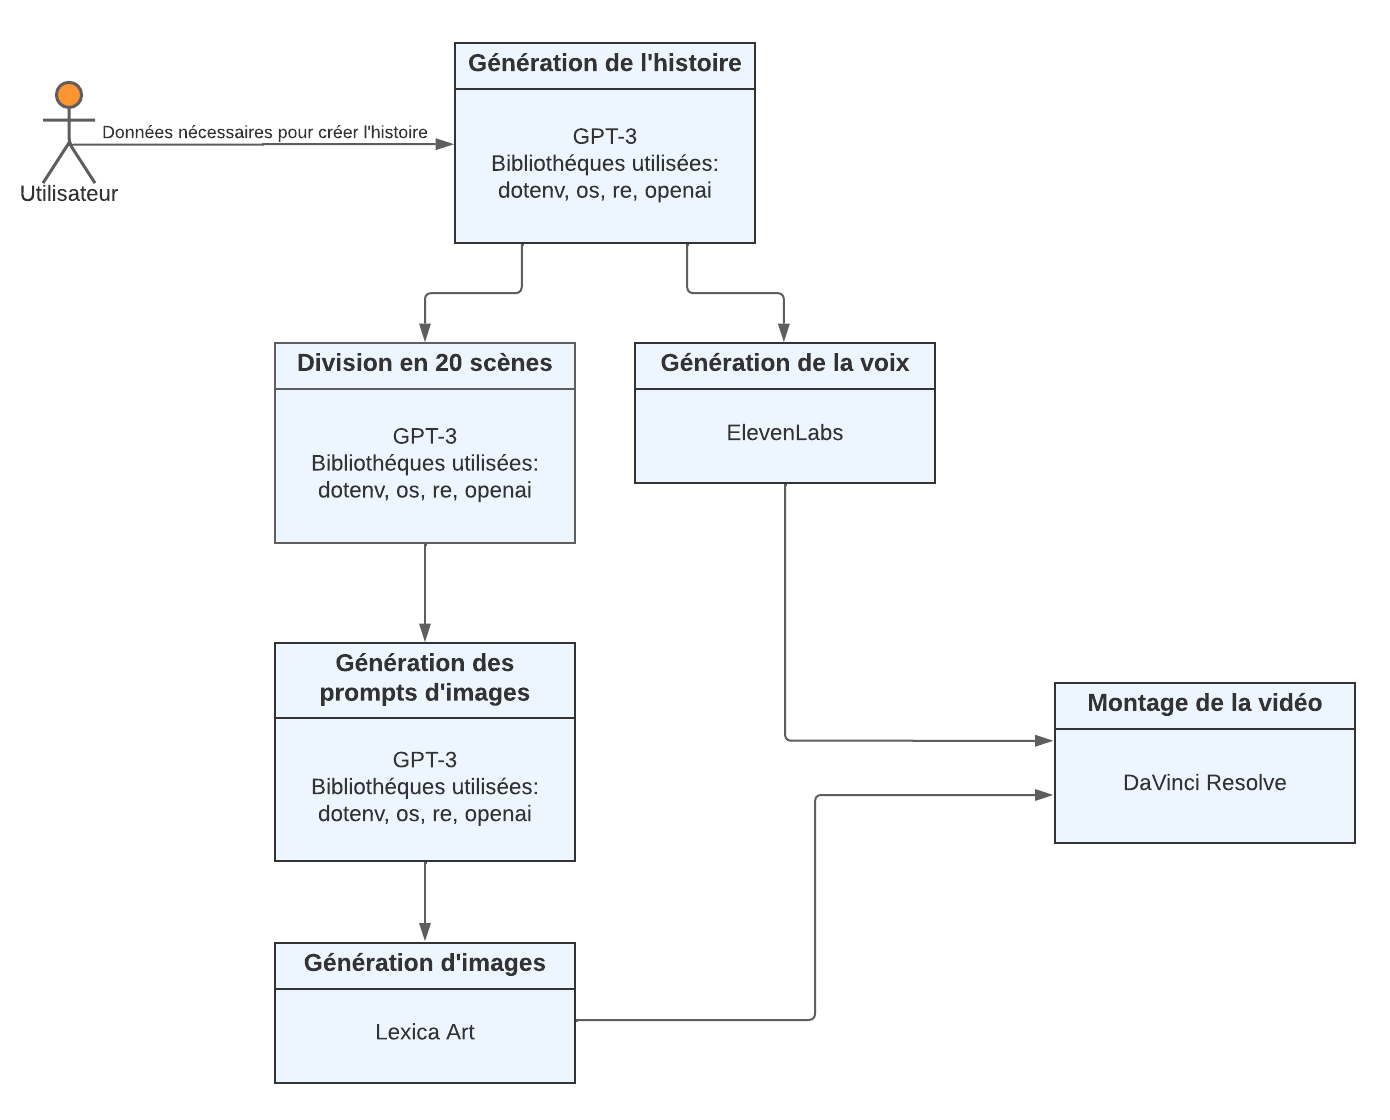
\includegraphics[keepaspectratio=true,scale=0.80]{images/diagram.png}}
	\captionof{figure}{Architecture technique du projet}   
\end{minipage}\\


\subsection{Technique de génération d'une bonne prompt}
Pour générer de bonnes prompts, il est important de respecter plusieurs critères :

\begin{enumerate}
  \item Langue correcte et idée claire et précise : Veillez à utiliser une langue correcte et à exprimer vos idées de manière claire et précise. Évitez les ambiguïtés ou les formulations confuses qui pourraient conduire à des résultats imprécis.
  
  \item Respectez la formule suivante : Une structure de prompt efficace peut être construite en suivant la formule : MEDIUM -> QUI -> FAIT QUOI ET OÙ -> STYLE D'IMAGE ET MOTS-CLÉS. Cette formule permet de donner des indications spécifiques sur le sujet, l'action, le lieu, le style d'image et les mots-clés pertinents.
  
  \item Positionnez les éléments importants en premier : Mettez en évidence les éléments les plus importants de votre prompt en les plaçant au début de la phrase. Cela permet au modèle d'IA de les prendre en compte en priorité et de générer des résultats correspondants.
  
  \item Utilisez des prompts négatives : Pour préciser ce que vous ne voulez pas dans la génération, vous pouvez également utiliser des prompts négatives. Par exemple, au lieu de dire "Je veux une image avec un ciel bleu", vous pouvez dire "Je ne veux pas une image avec un ciel nuageux".
\end{enumerate}

\subsection{Technique du Reverse Prompt Engineering}
Reverse Prompt Engineering\cite{RPE} est le processus de génération d'un prompt efficace à partir d'un texte existant en prenant en considération le style, la syntaxe, la langage et d'autres paramétres afin d'obtenir des résultats plus précis et adaptés aux besoins spécifiques de l'utilisateur. Les étapes à suivre sont comme suit : 
\begin{enumerate}
    \item Préselection : Lors de la présélection, les rétro-ingénieurs déterminent sur quoi ils vont tenter de travailler. Il peut s'agir d'un produit complet, d'un composant ou même d'un sous-composant.
    \item Désassemblage : La décompilation, également appelée désassemblage, est l'étape où le plus de travail se produit. À ce stade, les rétro-ingénieurs décomposent le produit qu'ils étudient. Ils tentent de rassembler toutes les informations et documentations possibles sur le fonctionnement du produit. Une fois qu'ils sentent qu'ils ont rassemblé toutes les pièces nécessaires, ils peuvent passer à l'étape suivante où ils essaient de les reconstituer.
    \item Vérification : Dans la troisième étape, les rétro-ingénieurs vérifient que toutes les pièces qu'ils ont découvertes au cours de la deuxième étape s'additionnent pour créer une réplique exacte de l'original. La réplique peut être testée pour s'assurer qu'elle produit les mêmes résultats que vous attendez de l'original.
    \item Création : Maintenant qu'une réplique fonctionnelle a été réalisée avec succès, les rétro-ingénieurs peuvent l'adapter et la modifier pour créer un nouveau produit doté de capacités plus avancées, ou peut-être la capacité de fonctionner avec différents systèmes non compatibles avec l'original.

\end{enumerate}

\chapter{Réalisation}
\section{Les outils et les technologies}

\subsection{GPT-3}\label{sec:GP}
GPT-3 (Generative Pre-trained Transformer 3) est un modèle de langage basé sur l'intelligence artificielle, développé par OpenAI. Il est considéré comme l'un des modèles de langage les plus avancés à ce jour. GPT-3 utilise une architecture de Transformer, qui est un type de réseau de neurones récurrents permettant de traiter des données séquentielles, comme des phrases ou des paragraphes.\newline

\begin{minipage}{\linewidth}
	\makebox[\linewidth]{
		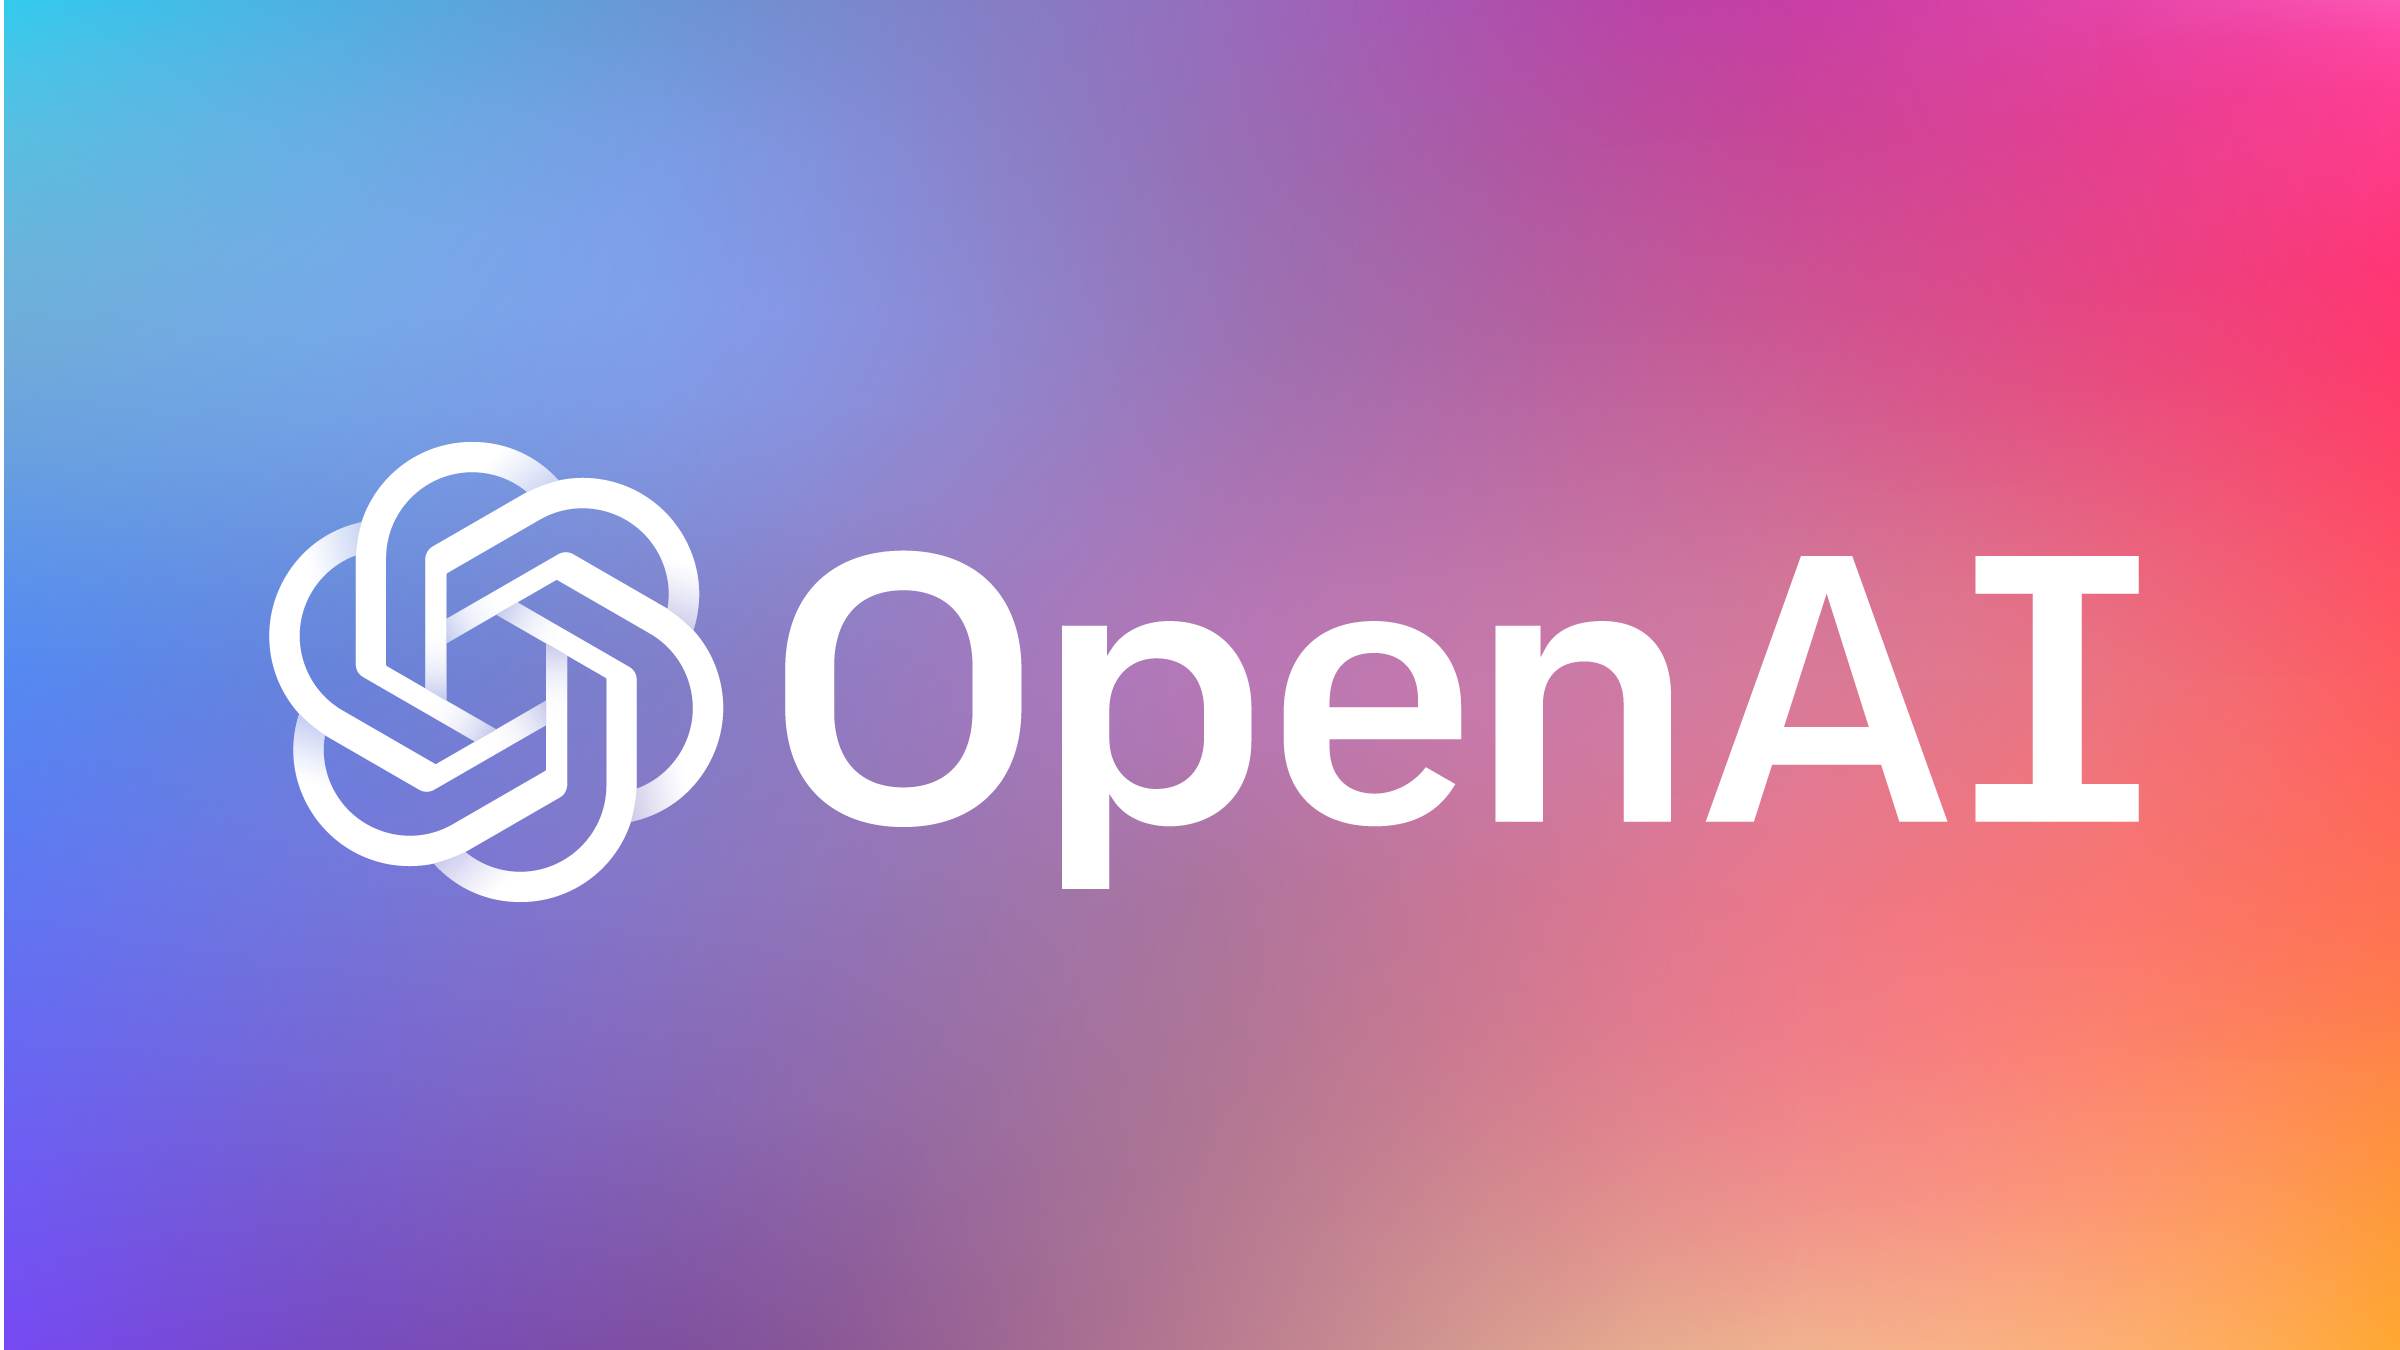
\includegraphics[keepaspectratio=true,scale=0.13]{images/openai.png}}
	\captionof{figure}{Pattern Openai GPT-3}\label{f3}%    
\end{minipage}\\

\subsection{Lexica art}\label{sec:Lex}
Lexica Art\cite{Lexica} est un générateur d'art AI qui utilise Stable Diffusion, un modèle de deep learning, text-to-image qui crée des images réalistes à partir des descriptions textuelles. Le modèle peut également être utilisé pour d'autres tâches, telles que la génération d'une image améliorée à partir d'un croquis et d'une description textuelle. \newline


\begin{minipage}{\linewidth}
	\makebox[\linewidth]{
		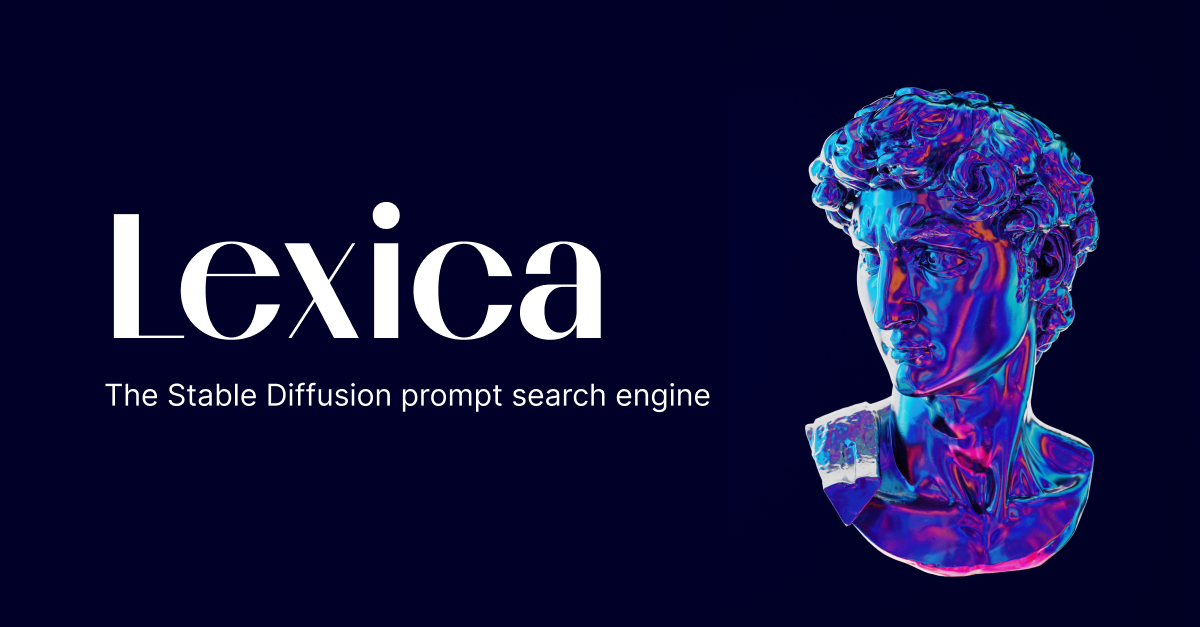
\includegraphics[keepaspectratio=true,scale=0.30]{images/lexica.png}}
	\captionof{figure}{Pattern Lexica art}\label{f3}%    
\end{minipage}\\

\subsection{ElevenLabs}\label{sec:El}
ElevenLabs\cite{ElevenLabs} est une entreprise qui fournit un service de text-to-speech, c'est-à-dire un logiciel qui prend du texte en entrée et produit une parole audible en sortie. La plupart des applications de text-to-speech utilisent une technologie basée sur l'OCR (reconnaissance optique de caractères), ce qui signifie qu'elles peuvent reconnaître les caractères dans les documents textuels ainsi que les images, et les transformer en parole.  \newline


\begin{minipage}{\linewidth}
	\makebox[\linewidth]{
		
\includegraphics[keepaspectratio=true,scale=0.3]{images/elevenlabs.png}}
	\captionof{figure}{Pattern ElevenLabs}\label{f3}%    
\end{minipage}\\
\subsection{DaVinci Resolve}\label{sec:dav}
DaVinci Resolve, développé par la société Blackmagic Design et auparavant par Da Vinci Systems, est un logiciel polyvalent de montage vidéo non linéaire, de mixage audio, de compositing et d'étalonnage. 

\begin{minipage}{\linewidth}
	\makebox[\linewidth]{
		
\includegraphics[keepaspectratio=true,scale=0.3]{images/davinci.png}}
	\captionof{figure}{Pattern DaVinci Resolve }\label{f3}%    
\end{minipage}\\

\subsection{Python}\label{sec:Py}
Python est un langage de programmation interprété, multiparadigme et multiplateformes. Il favorise la programmation impérative structurée, fonctionnelle et orientée objet. Python se distingue par son typage dynamique fort, sa gestion automatique de la mémoire par ramasse-miettes, ainsi que par son système de gestion d'exceptions. \newline


\begin{minipage}{\linewidth}
	\makebox[\linewidth]{
		
\includegraphics[keepaspectratio=true,scale=0.10]{images/python.png}}
	\captionof{figure}{Pattern Python}\label{f3}%    
\end{minipage}\\

\section{Analyse technique}
Le projet s'est déroulé en plusieurs phases distinctes durant desquelles nous avons utilisé des outlis spécifiques. Les étapes clés sont comme suit : 
\begin{enumerate}
    \item Génération du texte de l'histoire en utilisant l'API GPT-3 \hyperref[sec:GP]{d'OpenAI} et les bibliothéques \hyperref[sec:Py]{Python} suivantes : dotenv, os, re, \hyperref[sec:GP]{openai}, et ce en se basant sur les informations fournies par l'utilisateur décrivants l'histoire (personnages, lieux, ton, thème, etc).
    \item Division de l'histoire générée en 20 scènes en utilisant les mêmes outils utilisés dans la première étape.
    \item Génération des prompts destinées à la génération des images correspondantes à chaque scène de l'histoire en utilisant les même outils utilisés lors de la première phase.
    \item Génération des images avec \hyperref[sec:Lex]{Lexica Art}.
    \item Génération de la voix narratrice avec \hyperref[sec:El]{ElevenLabs}, un outil de synthèse vocale en ligne.
    \item Montage de la vidéo de l'histoire combinant les images générées ainsi que la voix narratrice avec \hyperref[sec:dav]{DaVinci Resolve} afin de créer une expérience immersive pour le spectateur.
\end{enumerate}

\section{Mise en oeuvre}

\subsection{Génération de l'histoire}
Dans la réalisation de notre projet, nous avons utilisé le langage de programmation Python pour générer automatiquement des histoires. Tout d'abord, nous importons les modules nécessaires, tels que "dotenv" pour charger les variables d'environnement à partir d'un fichier ".env", os pour accéder aux variables d'environnement, et "openai" pour interagir avec l'API d'OpenAI\cite{OpenAIDocs}\cite{OpenAIGit}.

Ensuite, nous chargeons la clé d'API d'OpenAI\cite{OpenAIDocs} à partir des variables d'environnement à l'aide de "load\_dotenv()" et "os.getenv()". Cette clé est utilisée pour authentifier notre demande à l'API.

Nous avons créé une fonction appelée split\_file qui nous permet de diviser le contenu d'un fichier texte en différentes parties. Cette fonction lit le fichier ligne par ligne et utilise des marqueurs spécifiques pour identifier les différentes parties de l'histoire, telles que le titre, le synopsis, les personnages, l'intrigue, etc. Les parties sont ensuite stockées dans un dictionnaire pour une utilisation ultérieure.

En utilisant la fonction split\_file, nous avons extrait les différentes parties de l'histoire à partir du fichier my\_story.txt, telles que le titre, le synopsis, les personnages, le genre, etc. Nous avons ensuite utilisé ces parties pour construire un prompt complet qui sera envoyé à l'API d'OpenAI\cite{OpenAIDocs} pour générer l'histoire.

Nous avons utilisé l'API d'OpenAI\cite{OpenAIDocs} pour générer l'histoire en fournissant le prompt que nous avons construit. Nous avons spécifié les paramètres de la requête, tels que le modèle à utiliser, le nombre maximum de mots dans l'histoire générée, la température pour contrôler le niveau de créativité, et l'arrêt pour indiquer quand l'histoire doit se terminer.

Une fois que nous avons reçu la réponse de l'API d'OpenAI\cite{OpenAIDocs}, nous avons extrait l'histoire générée et supprimé la partie du prompt qui se répétait. Ensuite, nous avons affiché l'histoire générée à l'écran et l'avons également sauvegardée dans un fichier texte appelé my\_generated\_story.txt pour une utilisation ultérieure.\newline


\subsection{Division de l'histoire en scènes}
Tout d'abord, nous avons lu l'histoire à partir du fichier my\_generated\_story.txt. Nous avons stocké le contenu de l'histoire dans une variable appelée story.

En utilisant cette histoire comme base, nous avons défini le prompt d'entrée pour l'API d'OpenAI\cite{OpenAIDocs}. Le prompt demande de diviser l'histoire en 20 scènes distinctes, en tenant compte de l'événement significatif, du changement de lieu ou du moment clé dans la progression de l'histoire. Nous demandons également une description détaillée de chaque scène.

Nous avons appelé l'API d'OpenAI\cite{OpenAIDocs} pour générer la division des scènes en utilisant le prompt que nous avons créé. Nous avons spécifié les paramètres de la requête, tels que le moteur à utiliser, le nombre maximum de jetons, la température pour contrôler le niveau de créativité et le nombre de réponses souhaitées (dans notre cas, 1).

Après avoir reçu la réponse de l'API, nous avons extrait la division des scènes générée à partir de la réponse. Nous l'avons ensuite séparée en scènes distinctes en utilisant le caractère de saut de ligne ("\textbackslash n").

Enfin, nous avons écrit les scènes dans un nouveau fichier appelé scenes\_division.txt. Chaque scène est écrite sur une nouvelle ligne, et nous avons également ajouté un saut de ligne après chaque scène pour une meilleure lisibilité.

\vspace{1cm}
\subsection{L'histoire finale et les scènes}

\textbf{L'histoire:}

\begin{center}
\textbf{The Scholar's Journal}
\end{center}


Chapter 1: The Discovery

Fatima had spent countless hours in dusty archives and ancient libraries, searching for clues about the scientific history of Morocco. But it wasn't until she stumbled upon a worn leather-bound journal in a small antique shop that her research truly came to life.

As she flipped through the pages of the journal, Fatima felt as though she had uncovered a hidden treasure. The journal was written by a Moroccan scholar from the past, and it was filled with detailed descriptions of scientific discoveries and innovations. Fatima was captivated by the scholar's passion for science, and she felt a kinship with him as she read about his struggles with discrimination and his determination to pursue knowledge despite the odds.

Determined to learn more about the scholar and his work, Fatima set out on a journey across Morocco. She traveled to different regions of the country, seeking out experts in various fields of science who could provide more information about the scholar's discoveries. Along the way, she met with astronomers, doctors, engineers, and other scientists, each of whom shared a piece of the puzzle that was the scholar's legacy.

Chapter 2: The Astronomy of Marrakesh

Fatima arrived in Marrakesh, the bustling city famous for its vibrant markets and ornate architecture. But she was not there for the souks or the palaces – she was there to learn about astronomy. She had read in the scholar's journal about his fascination with the stars and planets, and she hoped to find out more about the astronomy of Morocco's past.

She met with a local astronomer named Hassan, who took her on a tour of the city's ancient observatories. Hassan explained how the scholars of the past used intricate instruments to study the movements of the stars and planets, and how they used this knowledge to develop calendars and navigate the seas.

As Fatima listened to Hassan's explanations, she felt a sense of awe at the level of scientific knowledge that existed in Morocco's past. She realized that the scholar she had been reading about was not alone in his pursuit of scientific understanding – there were countless others like him who had dedicated their lives to unlocking the mysteries of the universe.

Chapter 3: The Medicine of Fez

Next, Fatima traveled to Fez, the ancient city known for its beautiful mosques and bustling souks. Here, she hoped to learn about the medical innovations of Morocco's past.

She met with a doctor named Aisha, who showed her around the city's old hospitals and clinics. Aisha explained how the scholars of the past had developed sophisticated medical techniques, using herbs and plants to treat a variety of ailments.

As Fatima listened to Aisha's explanations, she realized that the medical knowledge of Morocco's past was not only advanced but also deeply rooted in the country's culture and traditions. She understood how the scholar she had been reading about had been able to make such groundbreaking discoveries – he had been building on a foundation of knowledge that had been developed over centuries.

Chapter 4: The Engineering of Casablanca

Finally, Fatima arrived in Casablanca, the modern city known for its bustling port and towering skyscrapers. Here, she hoped to learn about the engineering innovations of Morocco's past.

She met with an engineer named Ahmed, who showed her around the city's construction sites and explained how the scholars of the past had used advanced engineering techniques to build impressive structures, such as aqueducts and mosques.

As Fatima listened to Ahmed's explanations, she realized that the engineering knowledge of Morocco's past was just as impressive as its astronomy and medicine. She felt a sense of pride in the accomplishments of her country's past and was inspired to continue her research, to learn even more about the scientific legacy of Morocco.

Chapter 5: The Legacy Continues

Fatima returned to her hometown, filled with a newfound appreciation for the scientific heritage of Morocco. She spent countless hours poring over the scholar's journal and the notes she had taken during her travels, piecing together a comprehensive picture of the scientific knowledge that had been developed in her country's past.

But she knew that her work was far from done. She wanted to share her findings with others, to inspire a new generation of scientists to build on the knowledge that had been developed in Morocco's past. And so, she began to teach, to hold lectures and workshops, to share her passion for science with anyone who would listen.

As she watched her students grow and develop their own scientific understanding, Fatima felt a sense of fulfillment. She knew that the legacy of Morocco's past was alive and well, that it was being carried forward by a new generation of curious minds.

And as she looked out over the city, watching as the sun set over the horizon, Fatima felt a sense of pride in her country's past and hope for its future. She knew that there was still so much to learn, so much to discover, but she was excited to be a part of that journey – to be a part of the ongoing legacy of Morocco's scientific history.
\newline

\textbf{Les scènes :}\newline

Scene 1: Fatima discovers the leather-bound journal in an antique shop.

Scene 2: Fatima reads through the journal and discovers the scholar's passion for science.

Scene 3: Fatima begins her journey across Morocco in search of experts in various fields of science.

Scene 4: Fatima arrives in Marrakesh and meets with an astronomer named Hassan.

Scene 5: Hassan takes Fatima on a tour of the city's ancient observatories.

Scene 6: Fatima is in awe of the level of scientific knowledge that existed in Morocco's past.

Scene 7: Fatima travels to Fez and meets with a doctor named Aisha.

Scene 8: Aisha shows Fatima around the city's old hospitals and clinics.

Scene 9: Fatima realizes the medical knowledge of Morocco's past is deeply rooted in the country's culture and traditions.

Scene 10: Fatima arrives in Casablanca and meets with an engineer named Ahmed.

Scene 11: Ahmed takes Fatima on a tour of the city's construction sites.

Scene 12: Fatima realizes the engineering knowledge of Morocco's past is just as impressive as its astronomy and medicine.

Scene 13: Fatima returns home and begins piecing together a comprehensive picture of the scientific knowledge of Morocco's past.

Scene 14: Fatima begins to teach, to share her passion for science with anyone who will listen.

Scene 15: Fatima watches her students grow and develop their own scientific understanding.

Scene 16: Fatima feels a sense of fulfillment in knowing her work is enabling the legacy of Morocco's past to be carried forward.

Scene 17: Fatima looks out over the city and is filled with pride in her country's past and hope for its future.

Scene 18: Fatima feels a renewed enthusiasm for her research and is excited to be a part of the ongoing legacy of Morocco's scientific history.

Scene 19: Fatima continues to search for new clues about Morocco's scientific history.

Scene 20: Fatima shares her findings with others, inspiring a new generation of scientists to build on the knowledge of Morocco's past.

\subsection{Génération des images}
\subsubsection{Création des prompts}
Dans cette partie, nous générons des prompt d'images AI en utilisant la bibliothèque OpenAI\cite{OpenAIDocs}\cite{OpenAIGit}.

En suivant les mêmes étapes initiales de la génération d'histoire.

Nous avons  une fonction appelée "generate\_image\_prompt()". Cette fonction prend un prompt, un fichier de sortie et un titre de prompt en tant que paramètres. Elle utilise l'API d'OpenAI\cite{OpenAIDocs} pour générer un prompt d'image AI à partir du prompt fourni. Le prompt d'image généré est ensuite écrit dans le fichier de sortie avec le titre du prompt.

Ensuite, nous chargeons les scènes à partir du fichier "scenes\_division.txt" dans une liste appelée "scenes".

Nous définissons également le nom du fichier de sortie où nous enregistrerons les prompts d'images AI, "image\_prompts.txt".

Ensuite, nous générons des prompts d'images AI pour chaque scène et chaque personnage. Pour chaque scène, nous générons une prompt d'image AI en utilisant le numéro de la scène et la description de la scène. Nous utilisons la fonction generate\_image\_prompt() pour générer la prompt d'image et l'écrire dans le fichier de sortie.

De même, pour chaque personnage, nous générons une prompt d'image AI en utilisant le nom du personnage, sa description et son rôle dans l'histoire. Nous utilisons à nouveau la fonction generate\_image\_prompt() pour générer la prompt d'image et l'écrire dans le fichier de sortie.

Ce processus nous permet de générer des prompts d'images AI pour chaque scène et chaque personnage de l'histoire, en capturant visuellement l'essence de ces éléments importants de l'intrigue.

\subsubsection{Exemples des images générées}
\vspace{1cm}
\begin{figure}[htbp]
  \centering
  \begin{tabular}{cc}
    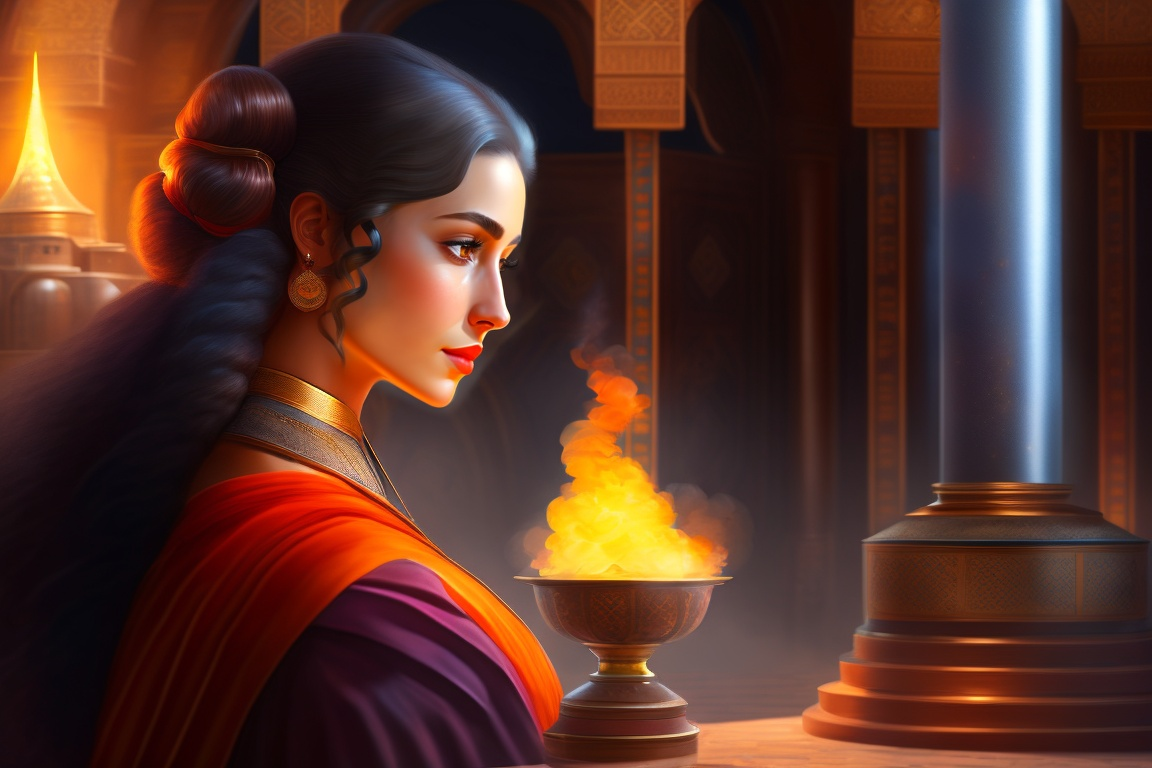
\includegraphics[width=0.5\textwidth]{images/image1.jpg} & 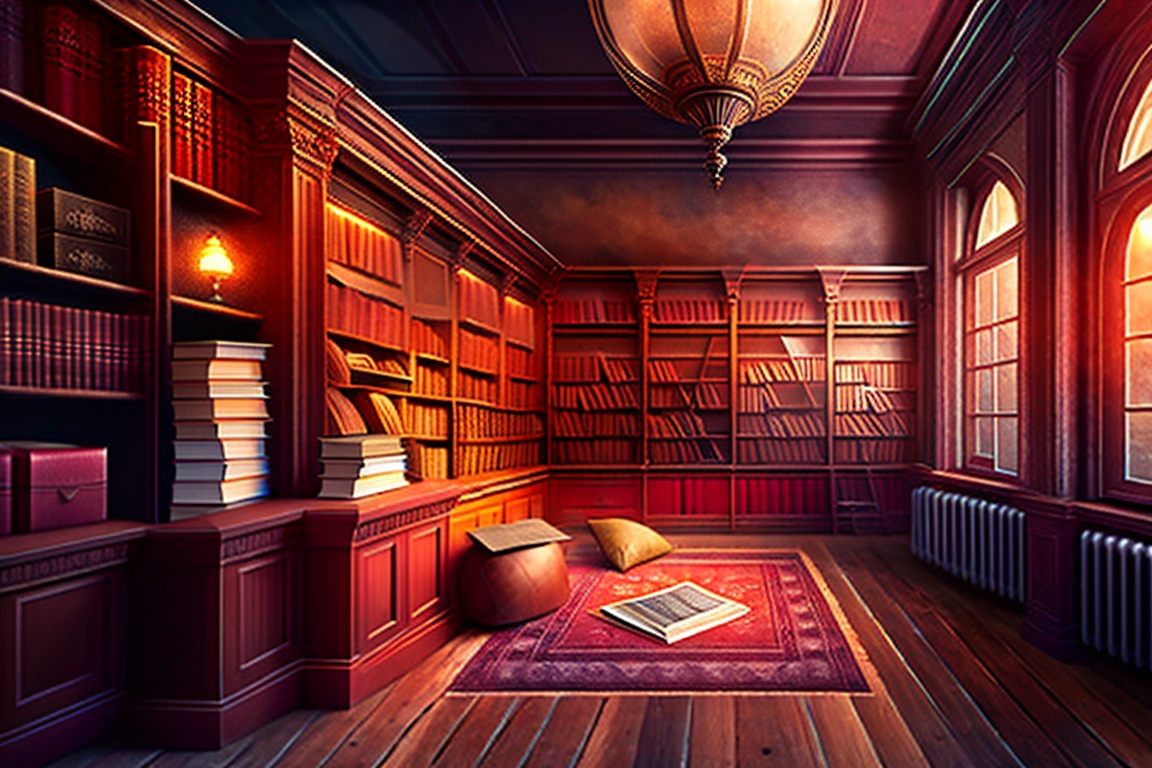
\includegraphics[width=0.5\textwidth]{images/image3.jpg} \\
    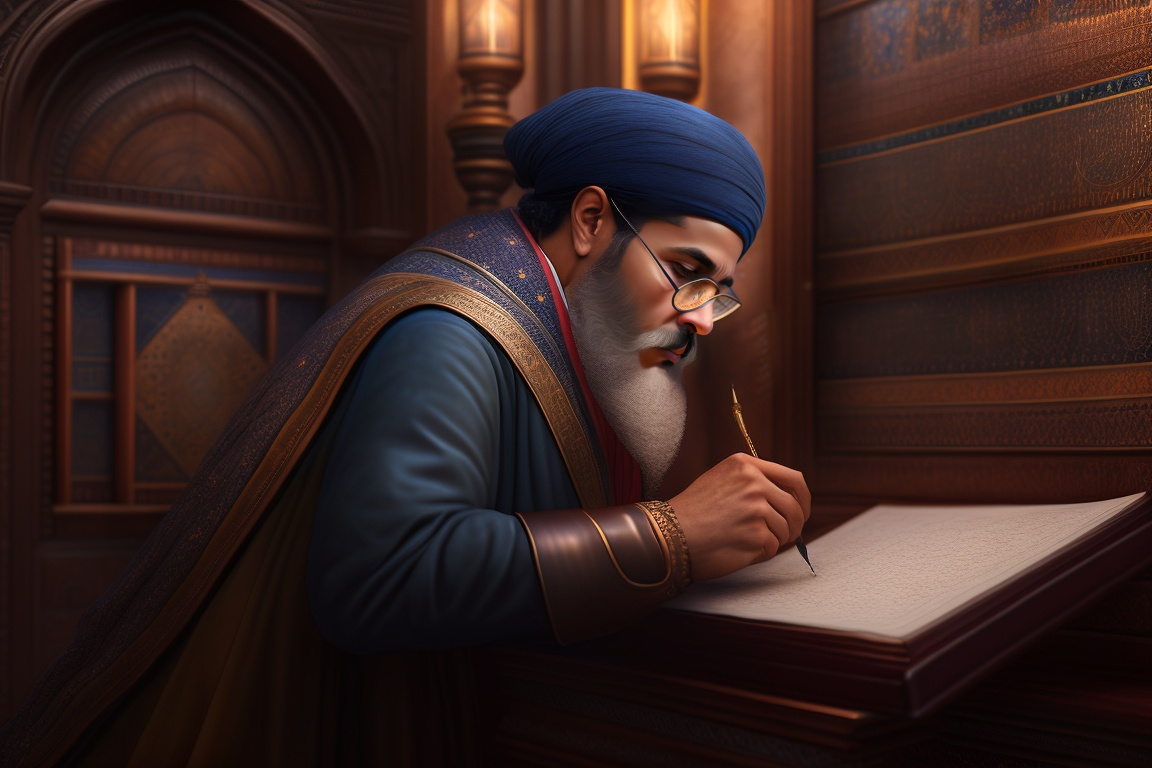
\includegraphics[width=0.5\textwidth]{images/image8.jpg} & 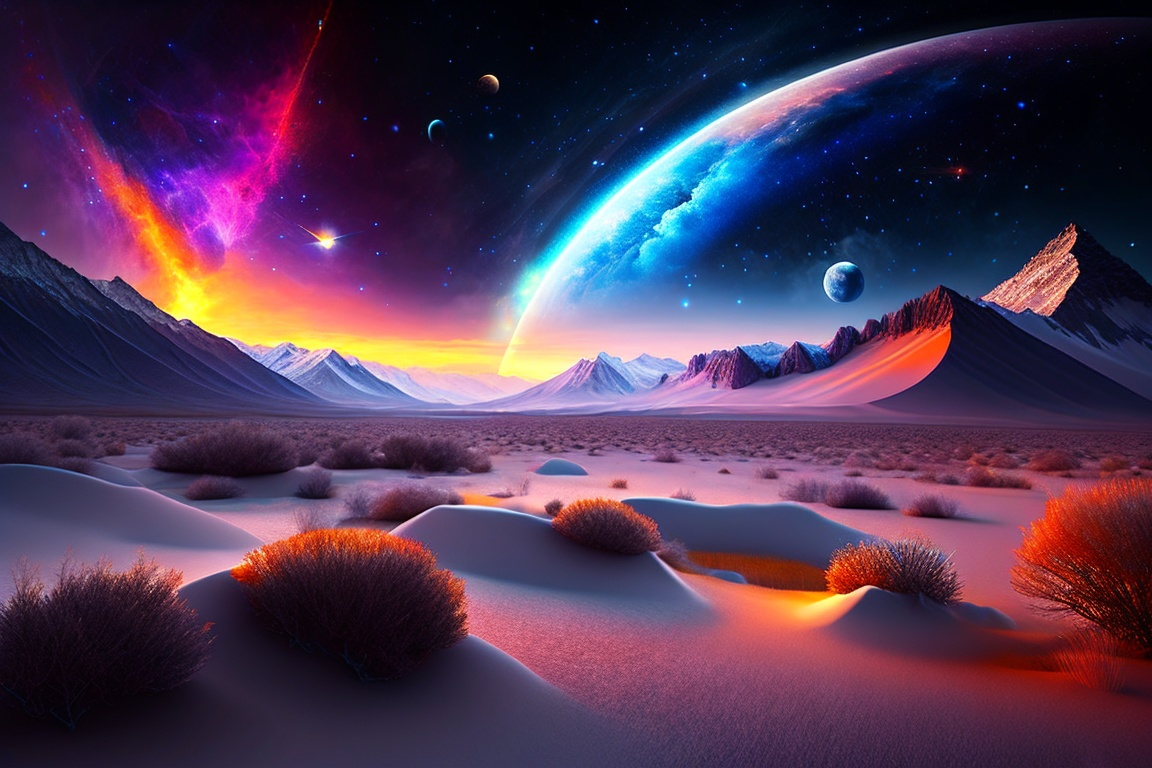
\includegraphics[width=0.5\textwidth]{images/image24.jpg} \\
  \end{tabular}
  \caption{Images générées}
  \label{fig:images}
\end{figure}



\cleardoublepage

\section{Problèmes rencontrés durant le projet}
\begin{spacing}{2}
\par 
L'un des principaux défis auxquels nous avons été confrontés lors de ce projet concerne les limitations des ressources disponibles. Étant donné que nous ne pouvions recourir qu’aux versions gratuites des outils utilisés, nous avons rapidement constaté des restrictions en termes de nombre de requêtes et d'accès aux fonctionnalités avancées, ce qui a eu un impact sur notre performance. Voici plus en détail les problèmes rencontrés :

\begin{itemize}
\item[•] \textbf{Implémentation des API :} Pour ce projet, nous avons utilisé l'API d'OpenAI\cite{OpenAIDocs}, cependant, une limitation majeure était le coût associé, car elle n'était  gratuite que pour un nombre limité de prompts. Cette contrainte a rendu l'exploration et la familiarisation avec la génération d'histoires plus difficiles. 
\item[•] \textbf{La génération des images:} Initialement, nous avions envisagé de travailler avec MidJourney, mais nous avons rencontré un problème : la génération d'une image nécessitait beaucoup de temps, notamment en raison de l'utilisation de la version gratuite de l'outil. Par conséquent, nous avons entrepris de rechercher d'autres IA similaires, offrant à la fois rapidité et gratuité. C'est ainsi que nous avons découvert Lexica Art\cite{Lexica}. Cependant, nous avons constaté que la qualité des images générées par Lexica Art\cite{Lexica} n'était pas aussi satisfaisante que celle produite par MidJourney.
\end{itemize}

\par
Il est à noter que ces limitations sont associées aux versions gratuites des outils utilisés et n’indiquent pas l’incapacité des technologies telles que GPT-3. Pour une utilisation plus optimale, il serait recommandé d'accéder aux versions payantes qui offrent des fonctionnalités plus étendues et mieux adaptées. Pour toute référence et détails sur le projet, veuillez accéder à notre projet sur GitHub. 

\footnotetext[\numexpr\thefootnote+1\relax]{lien vers projet : \href{https://github.com/GhitaLoukili/story-generation-with-python-and-gpt-3.git}{https://github.com/GhitaLoukili/story-generation-with-python-and-gpt-3.git}}

\appendix
\chapter*{Conclusion générale}
\addcontentsline{toc}{chapter}{Conclusion générale}
\markboth{Conclusion générale}{Conclusion générale}

\begin{onehalfspace}
Notre projet visait à explorer les différentes étapes de création d’histoires automatisées en utilisant l’API GPT-3 d’OpenAI\cite{OpenAIDocs}. Nous avons commencé par générer le texte en utilisant des bibliothèques Python et en établissant une communication avec l’API à travers des requêtes contenant des prompts décrivant les personnages, les situations, les lieux et d’autres détails concernant l’histoire souhaitée. l’API nous a renvoyé des réponses textuelles basées sur ces prompts. En suivant la même procédure, nous avons pu diviser l’histoire générée en 20 scènes et générer les prompts nécessaires pour les images de l’histoire. Par la suite, nous avons travaillé sur la génération d’images avec l’outil Lexica Art\cite{Lexica} pour obtenir les visuels correspondants à chaque scène de l’histoire. Puis nous avons eu recours à ElevenLabs\cite{ElevenLabs} pour la synthèse vocale. Ainsi nous avons pu créer une vidéo de l’histoire combinant les images générées et la voix narratrice.
\newline
L’utilisation de l’API GPT-3\cite{OpenAIDocs} nous a offert certes une certaine flexibilité et contrôle dans la génération du texte, mais n’empêche que ses avantages restent limités. En effet, les réponses générées peuvent parfois manquer de cohérence, de précision et de logique, ce qui a rendu la tâche difficile pour obtenir les résultats souhaités, particulièrement pour la génération des prompts des images.
\newline
Néanmoins, ce projet fut une opportunité pour nous familiariser avec les capacités de l’intelligence artificielle et prendre conscience de ses limites. En travaillant sur l’automatisation des étapes de création d'histoires, de la génération de textes à celle des images et de la voix, en utilisant GPT-3, Python et les autres outils, nous avons pu expérimenter au mieux ces technologies. Mais nous avons également dû faire face aux défis liés à l'utilisation de ressources gratuites, qui restreignent quelques fonctionnalités et performances.
\newline
Ce projet ouvre la perspective de construire une application qui automatise la création des histoires de manière plus interactive selon les préférences des utilisateurs. Elle pourrait inclure une interface conviviale où l’utilisateur fournirait les indications et détails de l’histoire souhaitée, et, en utilisant des modèles linguistiques avancés tels que GPT-4, l’application va générer une histoire complète. Elle pourrait également offrir la possibilité d’affiner l’histoire, et lui donner vie en générant des images et une voix narratrice choisie par l’utilisateur.
\newline
Mais en raison de l’évolution rapide des modèles d’IA générative, nous pouvons nous attendre à d’autres perspectives plus poussées. A titre d’exemple, les origines de GPT remontent à la fin de l’année 2017, et en seulement quelque année, GPT-3 fut introduite en 2020 ,qui se limitait à la génération du texte. Puis GPT-4 est arrivé en 2023, capable d’associer plusieurs sources de données (texte, voix, image, données) et d’appliquer des algorithmes de traitement\cite{BlogBus}. Cette progression témoigne de la rapidité de développement de ces modèles de langage. Il est en de même pour Midjourney, un modèle d’art génératif, dont le développement s’est déroulé en quelques mois, parmi de nombreux exemples similaires\cite{Blog}. Révolution ou évolution, l’IA générative ne cessera d’être un atout incontournable, malgré les différentes interrogations et limites auxquelles elle se retrouve confronté. On parle même de son exploitation dans les outils de développement low-code et no-code\cite{MondeInfo}, qui jouent déjà un rôle essentiel en aidant les utilisateurs professionnels à créer leurs propres applications, mais l’ajout d’une IA générative pourrait inciter encore plus à les adopter de manière plus élaborées.
\end{onehalfspace}


\renewcommand{\bibname}{Webographie}
\addcontentsline{toc}{chapter}{Webographie}

\begin{thebibliography}{6}
  
  \bibitem{OpenAIDocs}Documentation de l'API OpenAI : Documentation complète de l'API OpenAi. Date de la dernière consultation : 06/05/2023. Disponible sur : \href{https://platform.openai.com/docs/api-reference/introduction}{\nolinkurl{openai.com}}
  
  \bibitem{PromptGuide}Guide des prompts Phygital Plus Library : Guide détaillé sur l'utilisation des prompts dans la Phygital Plus Library .Date de la dernière consultation : 26/05/2023. Disponible sur : \href{https://library.phygital.plus/promptguide}{\nolinkurl{library.phygital.plus}}
  
  \bibitem{Chatgpt}OpenAI Chat : Plateforme de chat d'OpenAI, permettant d'interagir avec des modèles de langage et d'obtenir des réponses générées par l'IA. Date de la dernière consultation : 01/06/2023. Disponible sur : \href{https://chat.openai.com}{\nolinkurl{chat.openai.com}}
  
  \bibitem{OpenAIGit}Dépôt GitHub d'OpenAI Python : Dépôt GitHub contenant les bibliothèques et les exemples de code Python fournis par OpenAI. Date de la dernière consultation : 25/04/2023. Disponible sur : \url{https://github.com/openai/openai-python/tree/main}
  
  \bibitem{Lexica}Lexica Art :  Modèle de génération d'art. Date de la dernière consultation : 01/06/2023. Disponible sur : \href{https://lexica.art}{\nolinkurl{lexica.art}}
  
  \bibitem{ElevenLabs}Eleven Labs Speech Synthesis : Logiciel de synthèse vocale en ligne. Date de la dernière consultation : 26/05/2023. Disponible sur : 
  \href{https://beta.elevenlabs.io/speech-synthesis}{\nolinkurl{elevenlabs.io}}

  \bibitem{MondeInfo}Le Monde Informatique : L'IA générative va doper le développement Low-Code et No-Code. Date de la dernière consultation : 04/06/2023. Disponible sur : \href{https://www.lemondeinformatique.fr/actualites/lire-l-ia-generative-va-doper-le-developpement-low-code-et-no-code-90245.html}{\nolinkurl{lemondeinformatique.fr}}

  \bibitem{Blog}Blog du Modérateur : IA génératives : Comment ChatGPT et Midjourney vont impacter l'avenir. Date de la dernière consultation : 04/06/2023. Disponible sur : \href{https://www.blogdumoderateur.com/ia-generatives-comment-chatgpt-midjourney-vont-impacter-avenir/}{\nolinkurl{blogdumoderateur.com}}

  \bibitem{RPE}3D Engineering : Reverse Engineering Process Steps. Date de la dernière consultation : 04/06/2023. Disponible sur : \href{https://3d-engineering.net/reverse-engineering-process-steps/}{\nolinkurl{3d-engineering.net}}
  
\end{thebibliography}

\appendix
\chapter*{\fontsize{30}{18}\selectfont Annexe}
\addcontentsline{toc}{chapter}{Annexe}
\markboth{Annexe}{Annexe}

\begin{figure}[htbp]
    \centering
    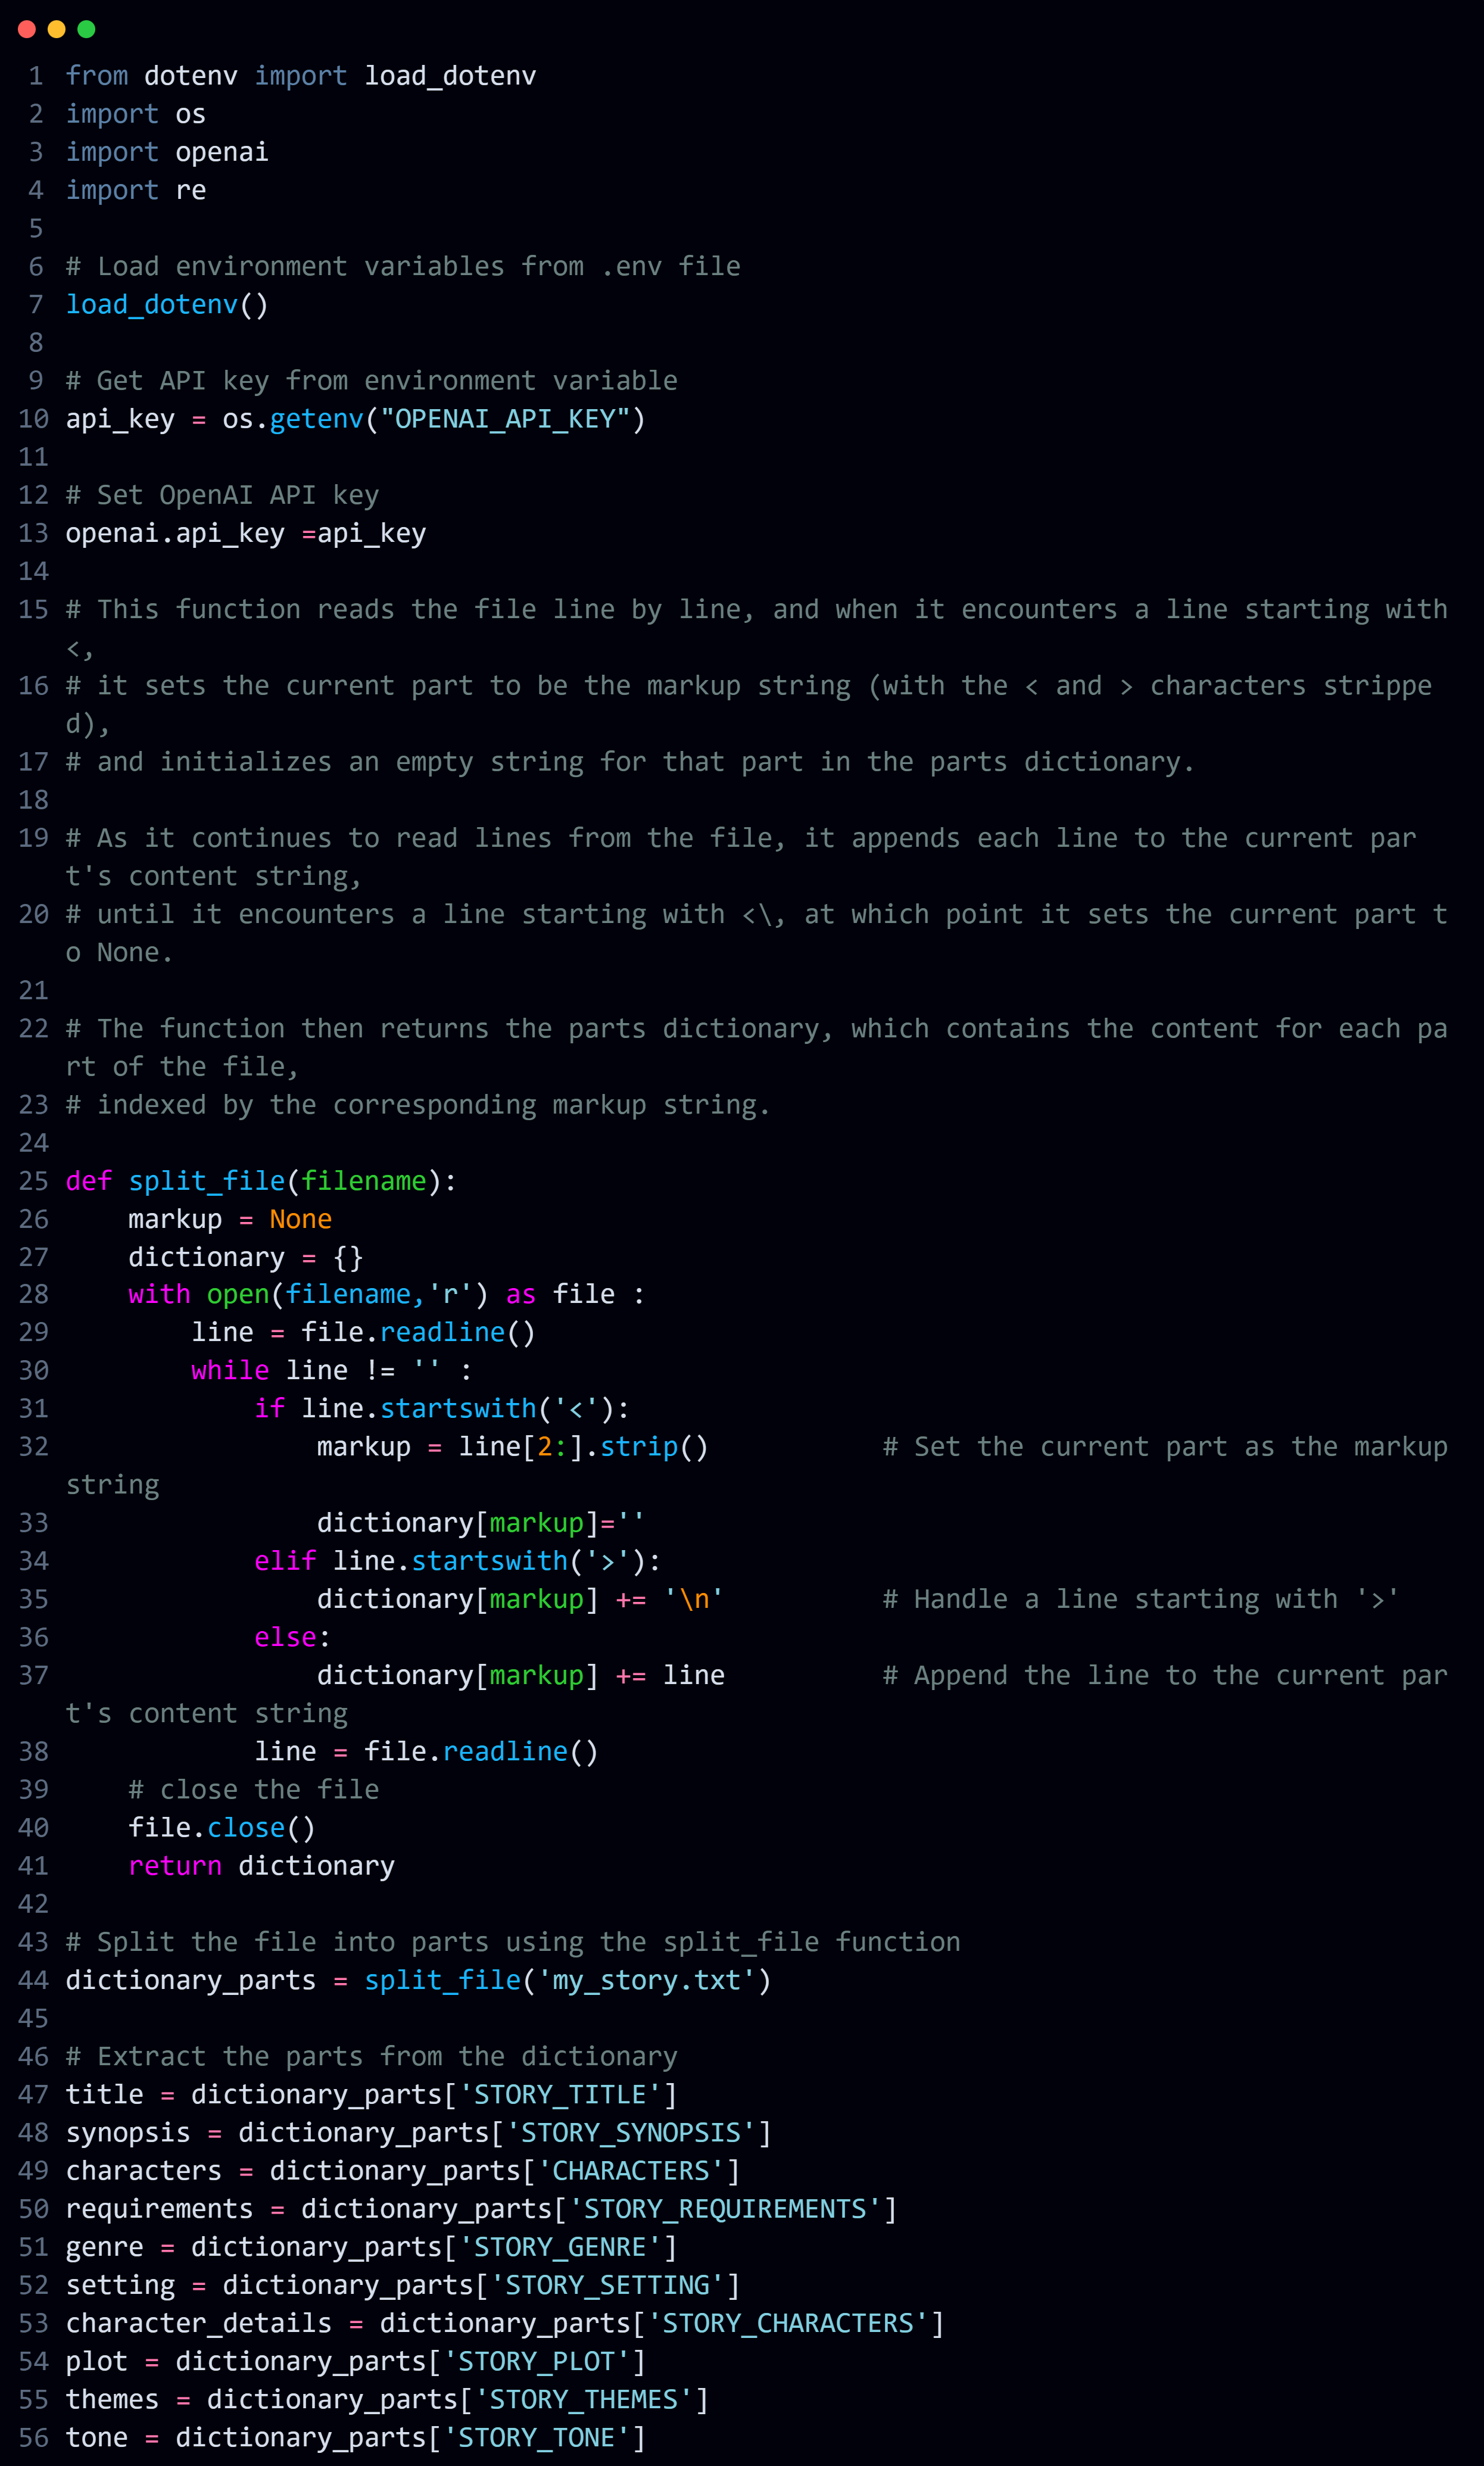
\includegraphics[keepaspectratio=true,scale=0.2]{images/creationScript1.png}
    \caption{Générateur de l'histoire (1)}
    \label{fig:generator1}
\end{figure}

\begin{figure}[htbp]
    \centering
    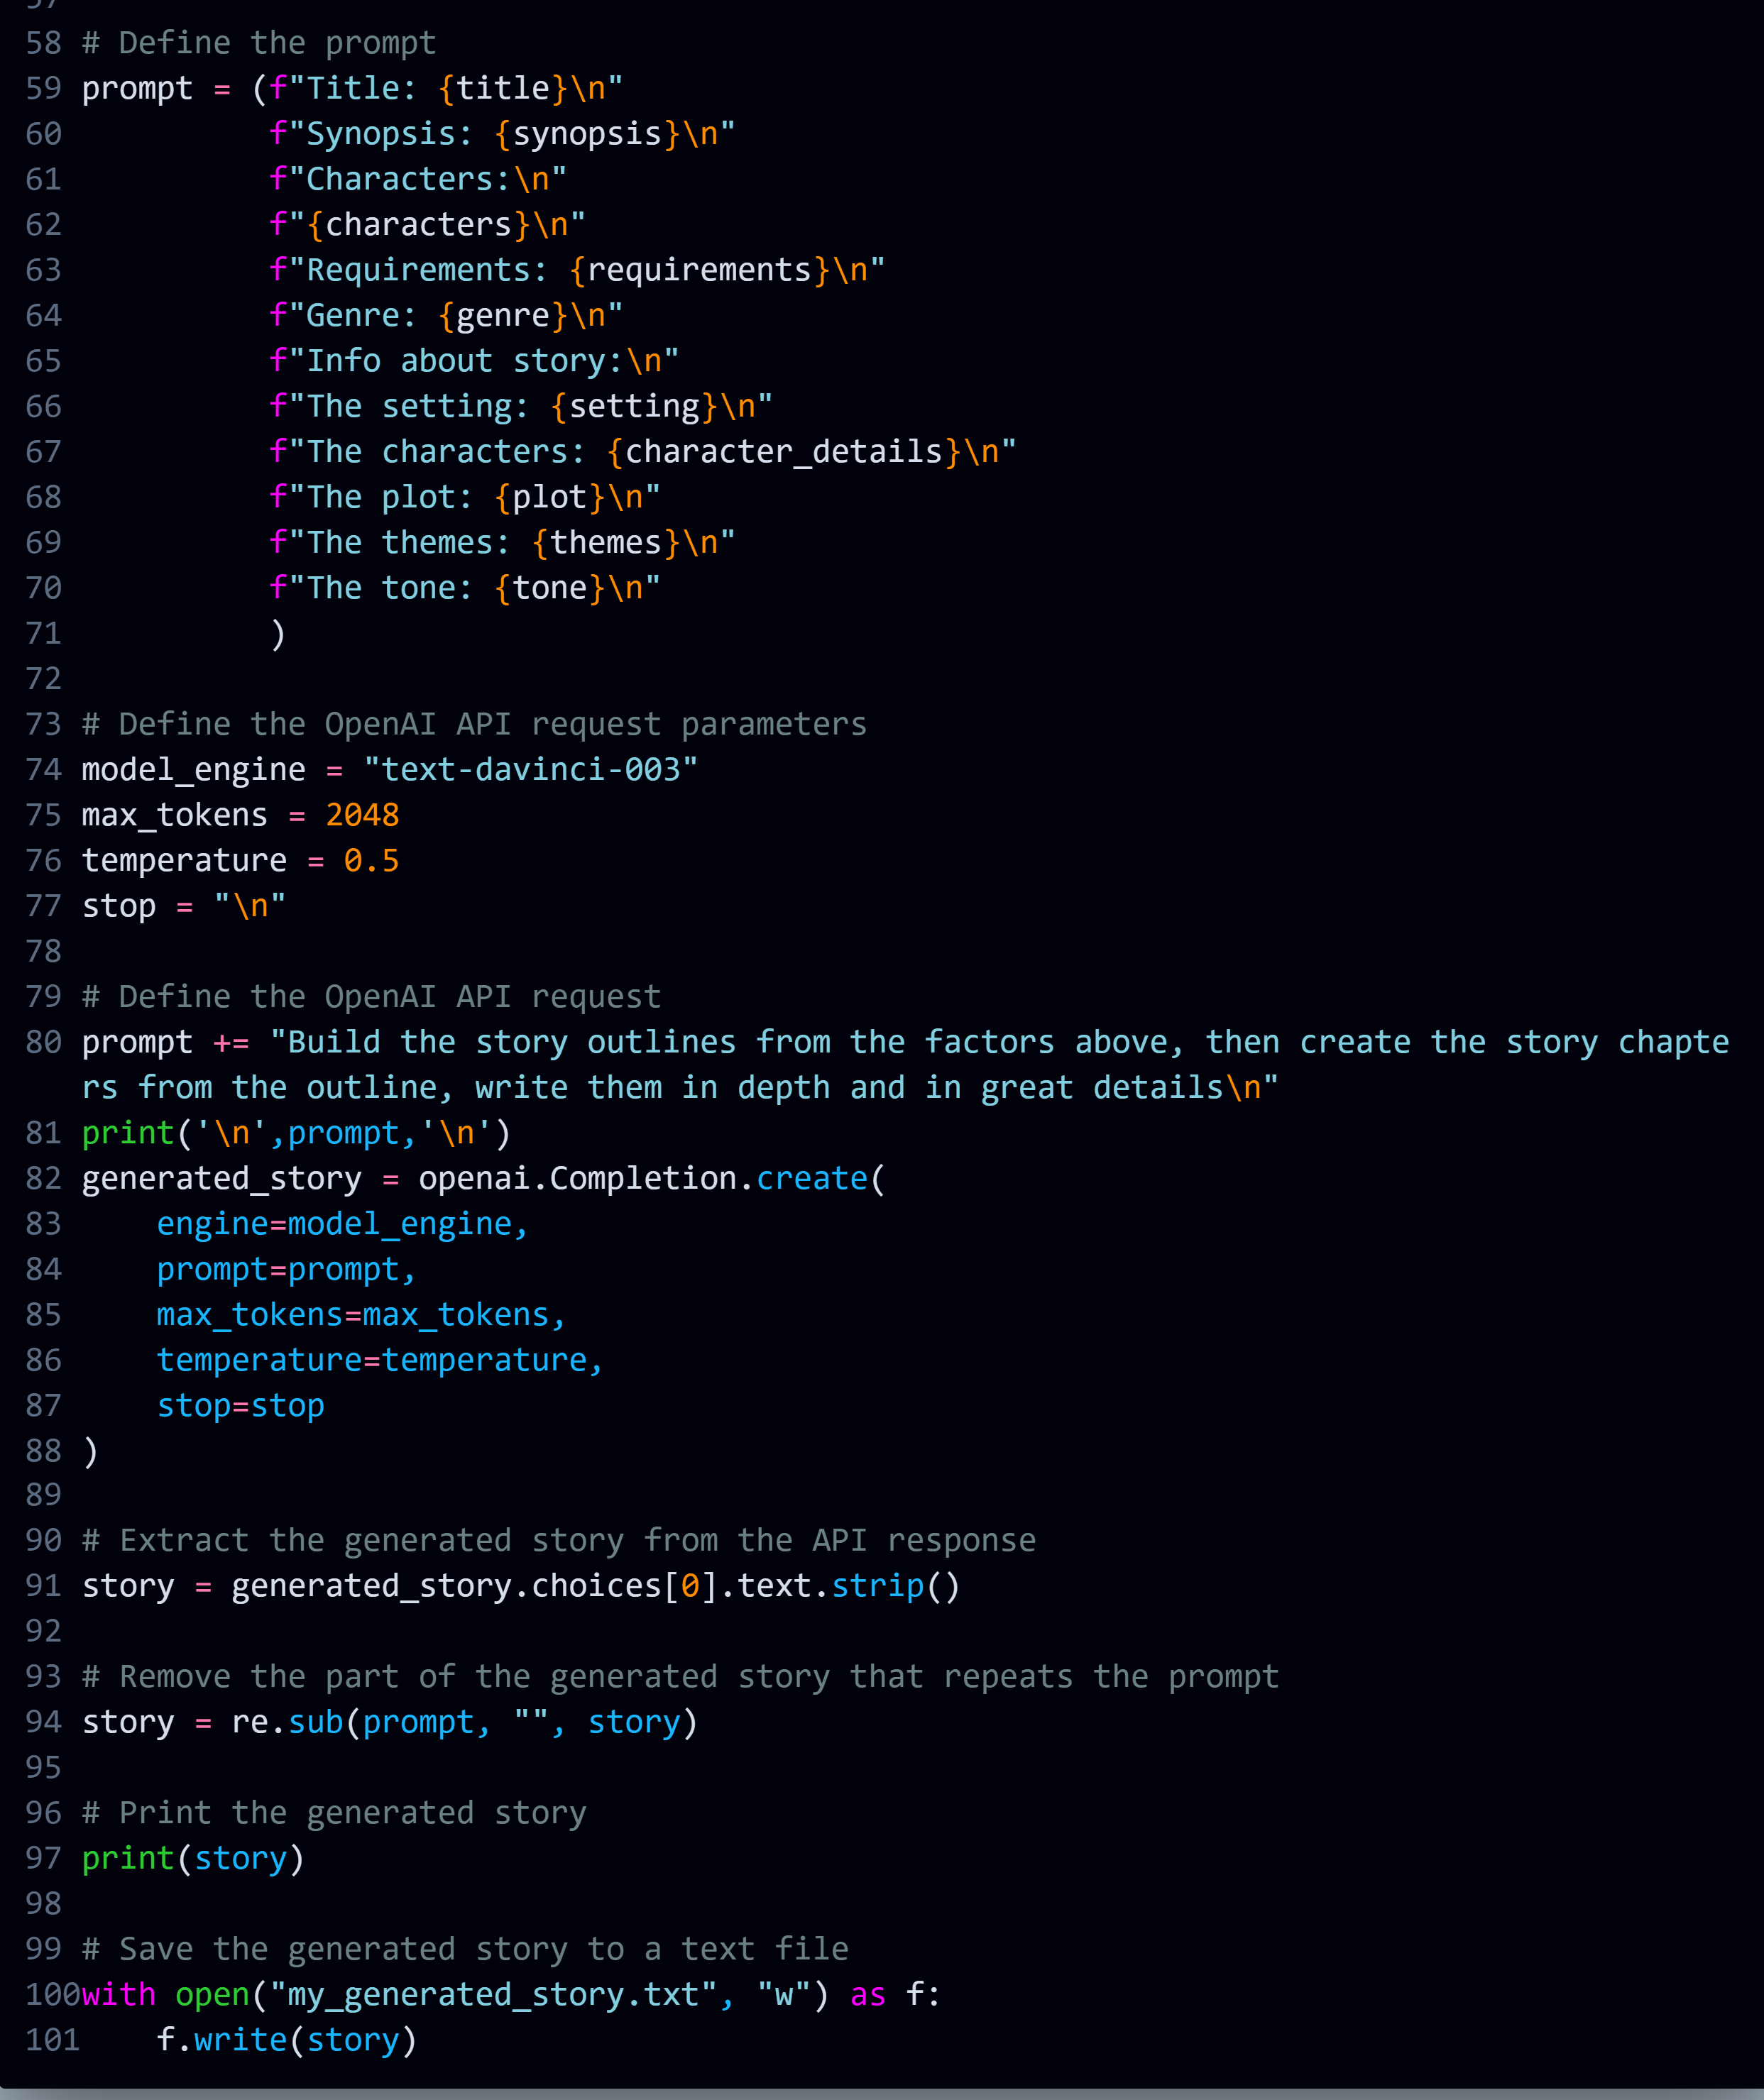
\includegraphics[keepaspectratio=true,scale=0.2]{images/creationScript2.png}
    \caption{Générateur de l'histoire (2)}
    \label{fig:generator2}
\end{figure}

\begin{figure}[htbp]
    \centering
    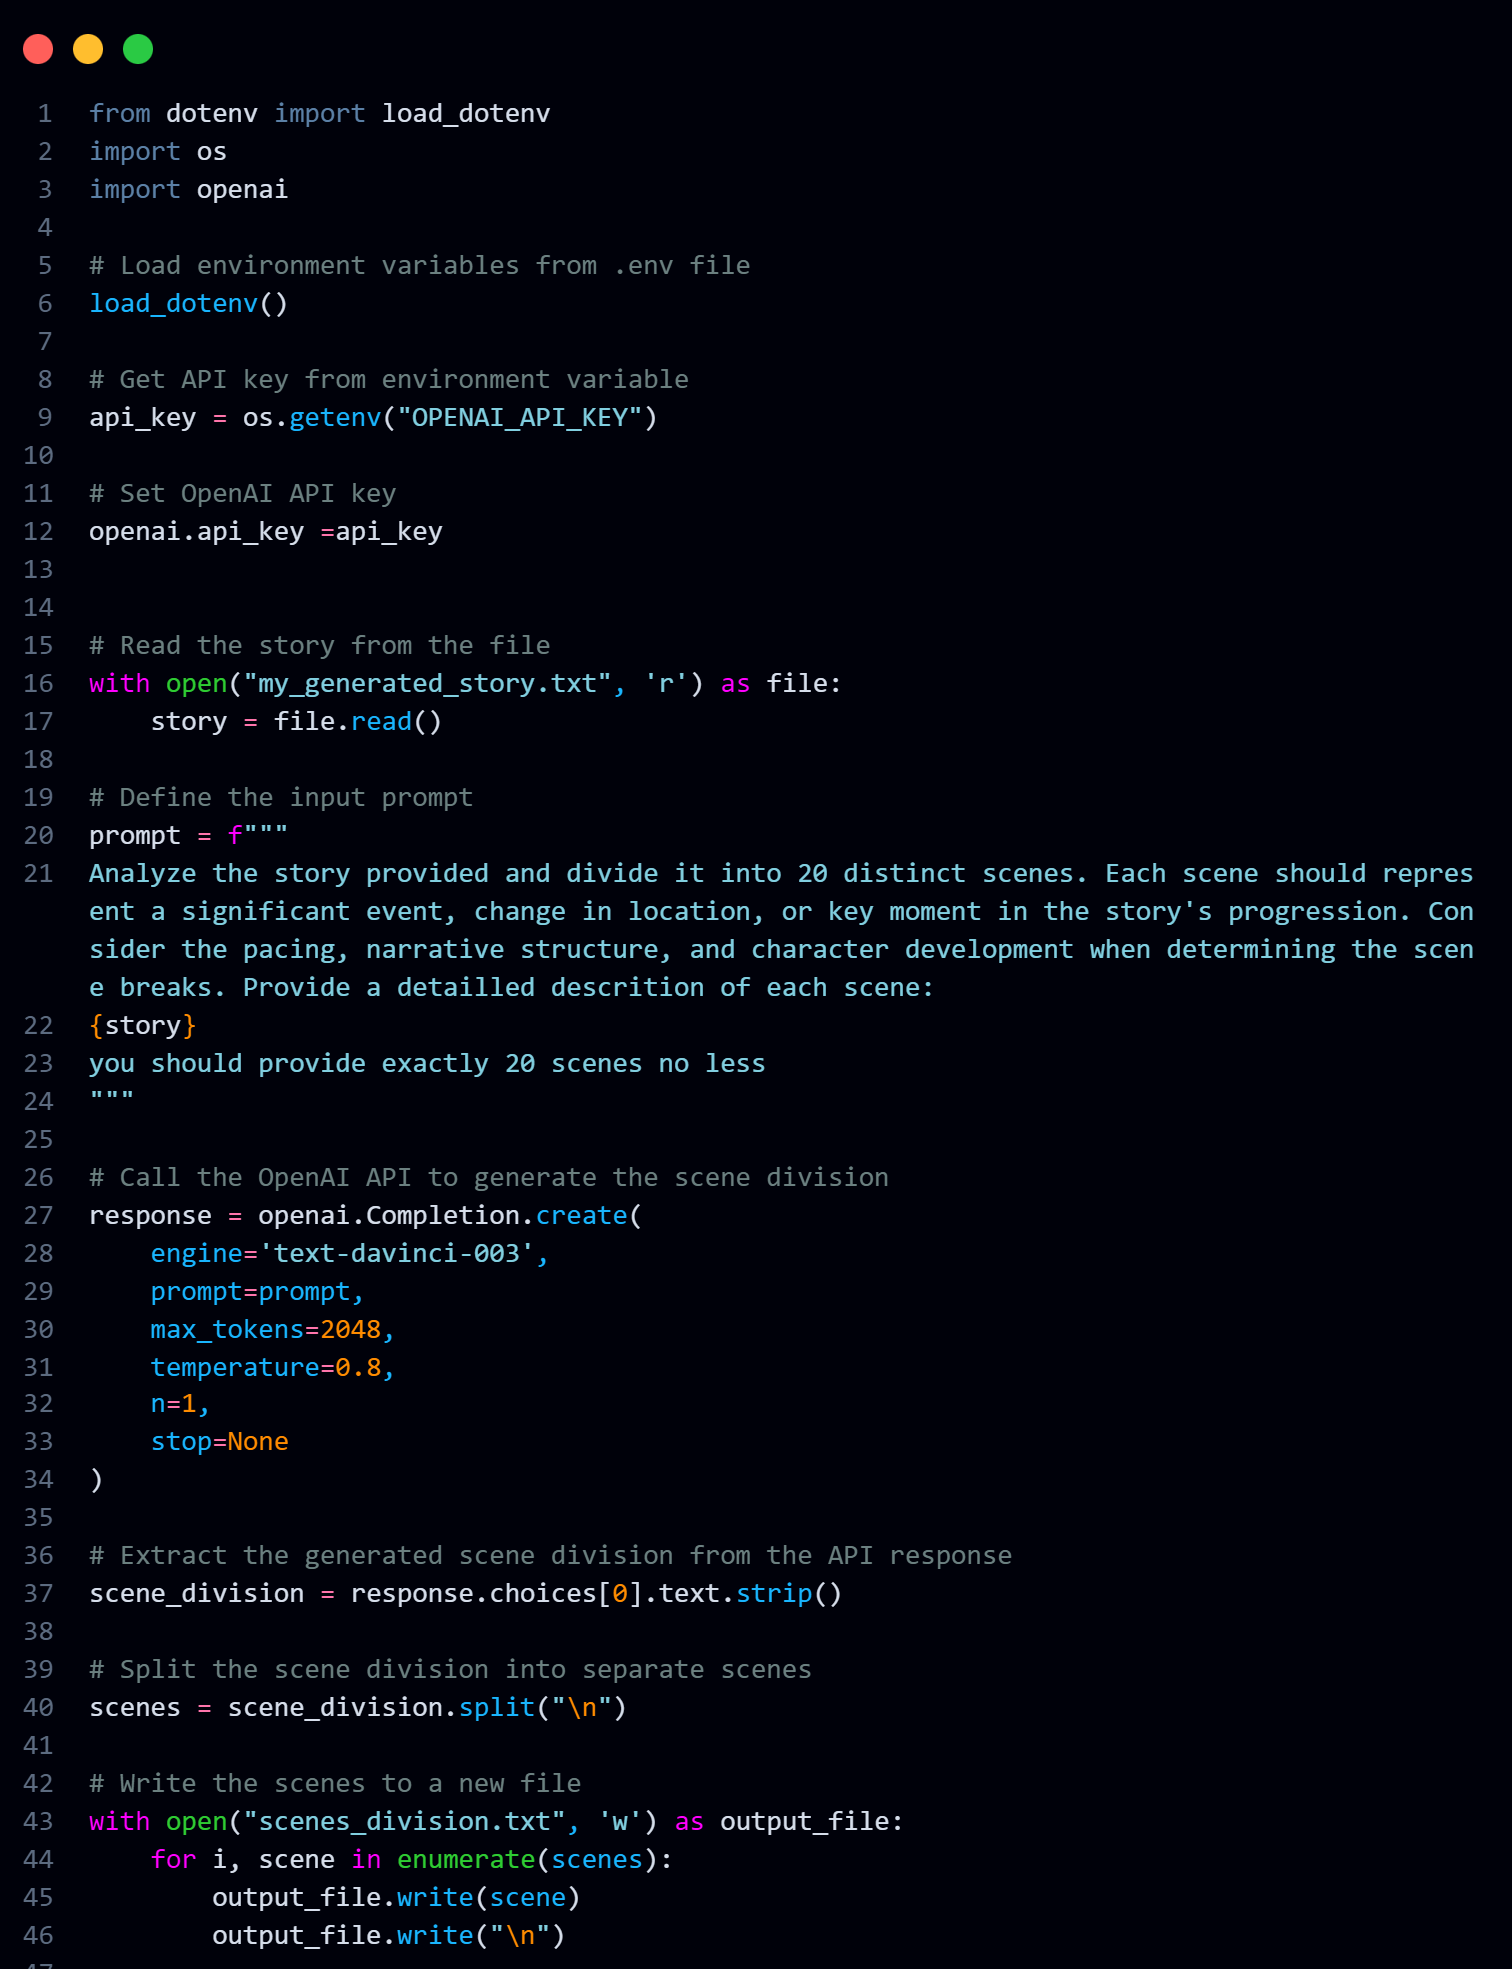
\includegraphics[keepaspectratio=true,scale=0.4]{images/division.png}
    \caption{Diviseur des scènes}
    \label{fig:dividor}
\end{figure}

\begin{figure}[htbp]
    \centering
    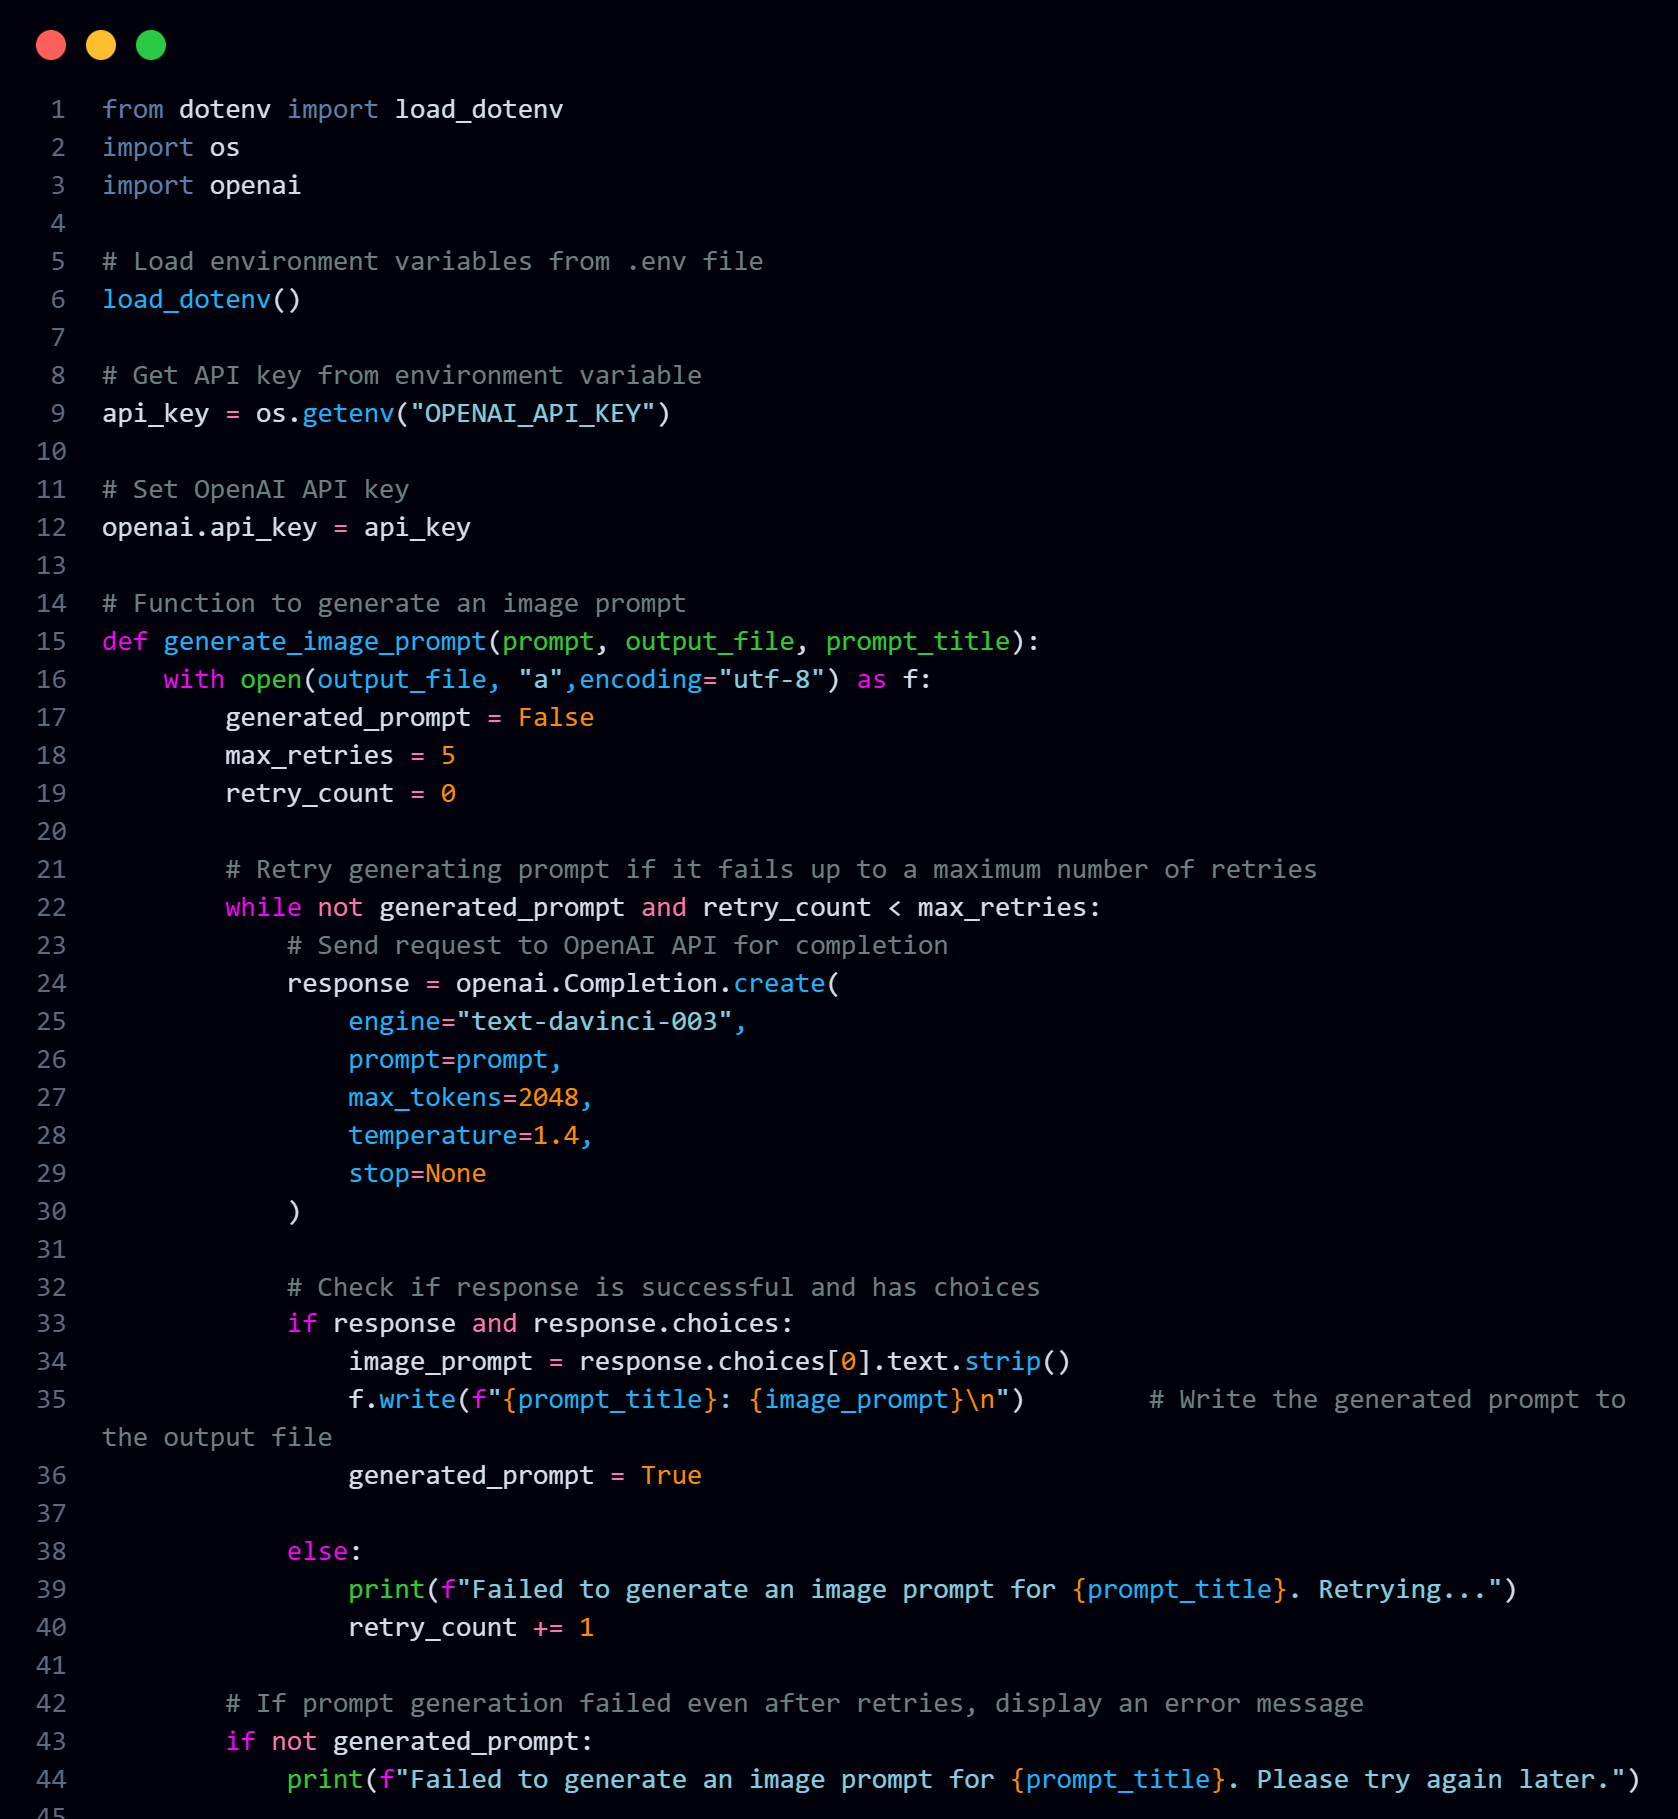
\includegraphics[keepaspectratio=true,scale=0.4]{images/promptfunction.png}
    \caption{Générateur de prompts (1)}
    \label{fig:p_generator1}
\end{figure}

\begin{figure}[htbp]
    \centering
    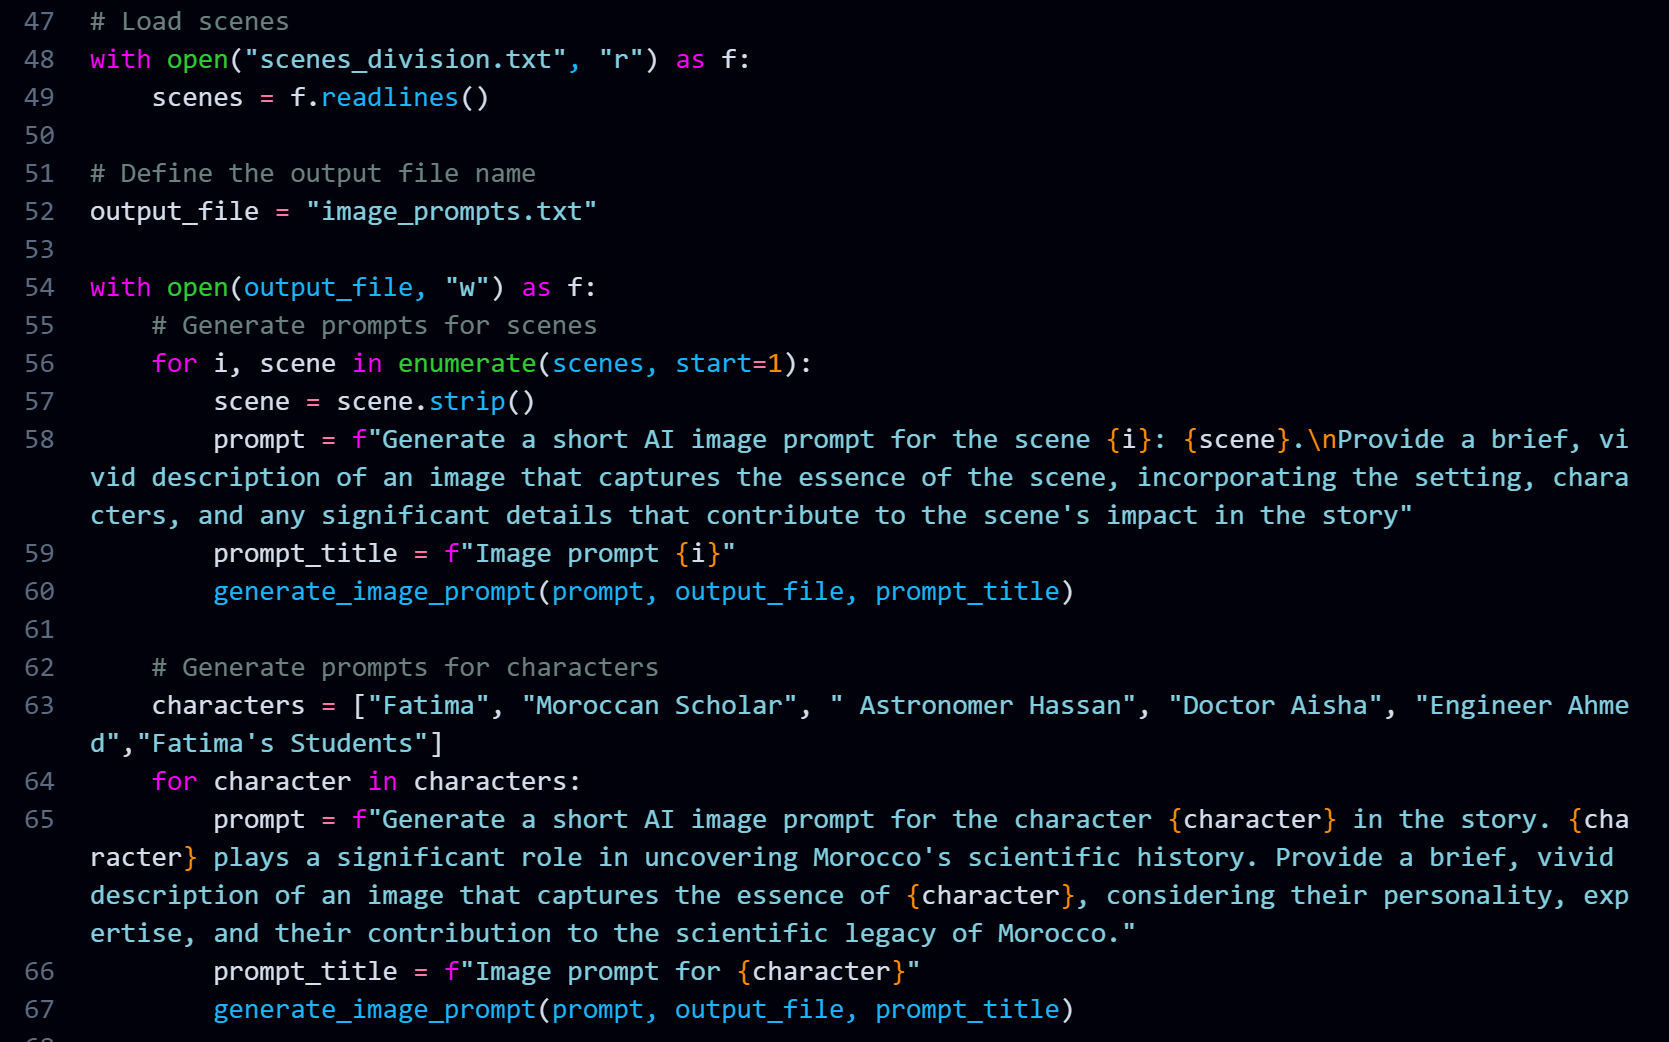
\includegraphics[keepaspectratio=true,scale=0.4]{images/image_prompt.png}
    \caption{Générateur de prompts (2)}
    \label{fig:p_generator1}
\end{figure}


\end{spacing}

\end{spacing}

\end{document}